\documentclass[sigconf,screen]{acmart}

\setlength{\pdfpagewidth}{8.5in}
\setlength{\pdfpageheight}{11.0in}

\usepackage{booktabs} % For formal tables
\usepackage{amsmath}
\usepackage{amssymb}
\usepackage{graphicx}
\usepackage{subfigure}
\usepackage[np,autolanguage]{numprint}
\usepackage{units}
\usepackage{fontawesome}
\usepackage{balance}
\usepackage{algorithm}
\usepackage[noend]{algorithmic}
\usepackage{color}
\setcitestyle{numbers,sort}

% math commands
\newcommand{\mat}[1]{\ensuremath{\mathbf{#1}}}
\newcommand{\card}[1]{\lvert #1\rvert}
\newcommand{\num}[1]{\numprint{#1}}

% unit commands
\newcommand{\h}{\unit{\,h}}
\newcommand{\s}{\unit{\,s}}
\newcommand{\ms}{\unit{\,ms}}
\newcommand{\bb}{\unit{\,B}}
\newcommand{\kb}{\unit{\,KB}}
\newcommand{\mb}{\unit{\,MB}}
\newcommand{\gb}{\unit{\,GB}}
\newcommand{\tb}{\unit{\,TB}}
\newcommand{\mbs}{\unit{\,MB/s}} %{~\unitfrac{MB}{s}}
\newcommand{\gbs}{\unit{\,GB/s}} %{~\unitfrac{GB}{s}} 
\newcommand{\gflop}{\unit{\,GFLOP}} %{~\unitfrac{GFLOP}{s}}
\newcommand{\gflops}{\unit{\,GFLOP/s}} %{~\unitfrac{GFLOP}{s}}
\newcommand{\tflops}{\unit{\,TFLOP/s}} %{~\unitfrac{TFLOP}{s}}

% algorithm commands
\renewcommand{\algorithmiccomment}[1]{\hfill \textit{// #1}}
\newcommand{\COMMENTLINE}[1]{\STATE \textit{// #1}}
\renewcommand{\algorithmicrequire}{\textbf{Input:}}
\renewcommand{\algorithmicensure}{\textbf{Output:}}
\renewcommand{\algorithmicrepeat}{\textbf{do}}
\renewcommand{\algorithmicuntil}{\textbf{while}}

%\SetKwRepeat{Do}{do}{while}
%\SetKwInOut{Input}{Input}\SetKwInOut{Output}{Output}

% format specific commands
\newenvironment{itemize2}{\begin{itemize}\setlength{\itemsep}{2.5pt}\setlength{\parskip}{0pt}\setlength{\parsep}{0pt}}{\end{itemize}}
\newenvironment{equation2}{\begin{equation}\small}{\end{equation}\hspace{-0.1cm}}

\setlength{\textfloatsep}{9pt}
\newtheorem{example}{Example}

\clubpenalty = 10000
\widowpenalty = 10000
\sloppy
\frenchspacing
%\pagenumbering{arabic}

\hyphenation{ExDRa}
\hyphenation{SystemDS}
\hyphenation{NebulaStream}
\hyphenation{MLog-Reg}
\hyphenation{off-line}


\AtBeginDocument{%
  \providecommand\BibTeX{{%
    \normalfont B\kern-0.5em{\scshape i\kern-0.25em b}\kern-0.8em\TeX}}}

%provided meta data
\copyrightyear{2021}
\acmYear{2021}
\setcopyright{acmlicensed}
\acmConference[SIGMOD '21]{Proceedings of the 2021 International Conference on Management of Data}{June 20--25, 2021}{Virtual Event, China}
\acmBooktitle{Proceedings of the 2021 International Conference on Management of Data (SIGMOD '21), June 20--25, 2021, Virtual Event, China}
\acmPrice{15.00}
\acmDOI{10.1145/3448016.3457549}
\acmISBN{978-1-4503-8343-1/21/06}

\settopmatter{printacmref=true}
\begin{document}
\fancyhead{}

%%%%%%%%%%%%%%%%%%%%%%%%%%%%%%%%%%%%%%%%%%%%%%%%%%%%%%%%%%%%%%%%%%%%%%%%%%%%%%%%%%%%%%%%%%%%%%%%%%%%
\title{ExDRa: Exploratory Data Science on Federated Raw Data}

\author{Sebastian Baunsgaard$^3$,
Matthias Boehm$^3$,
Ankit Chaudhary$^4$,
Behrouz Derakhshan$^2$}
\author{Stefan Gei{\ss}els{\"o}der$^1$,
Philipp M. Grulich$^4$,
Michael Hildebrand$^1$,
Kevin Innerebner$^3$}
\author{Volker Markl$^{2,4}$,
Claus Neubauer$^1$,
Sarah Osterburg$^1$,
Olga Ovcharenko$^3$,
Sergey Redyuk$^4$}
\author{Tobias Rieger$^3$,
Alireza Rezaei Mahdiraji$^2$,
Sebastian Benjamin Wrede$^3$,
Steffen Zeuch$^2$}
\affiliation{\vspace{0.15cm}\textsuperscript{1} Siemens AG;~~Berlin/Erlangen, Germany} 
\affiliation{\textsuperscript{2} DFKI GmbH;~~Berlin, Germany}
\affiliation{\textsuperscript{3} Graz University of Technology;~~Graz, Austria}
\affiliation{\textsuperscript{4} Technische Universit{\"a}t Berlin;~~Berlin, Germany\vspace{0.15cm}}

\renewcommand{\shortauthors}{Baunsgaard et al.}

\begin{abstract}
%1. State the problem
Data science workflows are largely exploratory, dealing with under-specified objectives, open-ended problems, and unknown business value. Therefore, little investment is made in systematic acquisition, integration, and pre-processing of data.
%2. Say why it's an interesting problem
This lack of infrastructure results in redundant manual effort and computation. Furthermore, central data consolidation is not always technically or economically desirable or even feasible (e.g., due to privacy, and/or data ownership).
%3. Say what your solution achieves
The ExDRa system aims to provide system infrastructure for this exploratory data science process on federated and heterogeneous, raw data sources. Technical focus areas include (1) ad-hoc and federated data integration on raw data, (2) data organization and reuse of intermediates, and (3) optimization of the data science lifecycle, under awareness of partially accessible data. In this paper, we describe use cases, the overall system architecture, selected features of SystemDS' new federated backend (for federated linear algebra programs, federated parameter servers, and federated data preparation), as well as promising initial results.
%4. Say what follows from your solution 
Beyond existing work on federated learning, ExDRa focuses on enterprise federated ML and related data pre-processing challenges. In this context, federated ML has the potential to create a more fine-grained spectrum of data ownership and thus, even new markets.
\end{abstract}

\maketitle


%%%%%%%%%%%%%%%%%%%%%%%%%%%%%%%%%%%%%%%%%%%%%%%%%%%%%%%%%%%%%%%%%%%%%%%%%%%%%%%%%%%%%%%%%%%%%%%%%%%%
\section{Introduction}

\textbf{Data Science Workflows:} Typical data science projects deal with open-ended questions, aiming to find patterns and predictive models that create business value \cite{BoehmADGIKLPR20}. Data scientists acquire samples for the given problem, and then enrich, clean, and prepare these data for model building and hypothesis testing \cite{CohenDDHW09}. This process is largely exploratory, where analysis results guide the incremental refinement of ML pipelines \cite{DerakhshanMARM20,XinMMLSP18}. Due to the unknown value and exploratory character---in stark contrast to traditional data warehousing \cite{CohenDDHW09}---little investment is made in systematic data acquisition, integration, and pre-processing \cite{SculleyHGDPECYC15}.

\textbf{Query Processing on Raw Data:} The inspiring work on query processing on raw data \cite{AlagiannisBBIA12,IdreosAJA11,KarpathiotakisA16} supports exploratory data analysis by executing SQL queries directly on raw data files. Repeated data access overhead is alleviated with dedicated caching strategies, positional maps for partial parsing, partitioning, and code generation. However, executing entire ML pipelines on raw data---with data cleaning and model training---remains an open problem.

\textbf{Data Ownership and Privacy:} Besides the exploratory character, a second major challenge is the limited access to data sources relevant to the given business problems. First, privacy-preserving data storage may not allow for central data consolidation. Similarly, in geo-distributed applications, central data consolidation can be economically or technically infeasible \cite{VulimiriCGKV15}. Second, data ownership limitations restrict the scope of data enrichment and consolidation. 
\begin{example}[Data Ownership Dilemma]
Consider a scenario of a machine vendor, a middle person who uses provided machines to test customer equipment, and customers. Any one of these stakeholders has vested interest in owning the detailed test measurements. The machine vendor wants to model and improve operations; the customer does not want to reveal equipment characteristics; and the middle person wants to offer data-driven products to various customers. 
\end{example}
\noindent Therefore, data ownership and sharing agreements are usually negotiated in bilateral contracts among stakeholders. In the context of exploratory data science, these access limitations are, however, challenging because the return on investment (e.g., impact on predictions) of data purchases or subscriptions is unknown upfront.

\textbf{Federated ML:} Recent work on federated learning \cite{BonawitzEGHIIKK19} partially addresses this problem of inaccessible data. Federated ML learns a global model without central data consolidation, for example, on private data of mobile devices. Existing work adopts a traditional parameter server architecture \cite{SmolaN10,DeanCMCDLMRSTYN12,LiAPSAJLSS14,JiangCZY17}. The parameter server initializes and broadcasts a model, every client device now acts as a worker, computes gradients over mini-batches of their local data (e.g., via a forward and backward pass through a neural network), and pushes these gradients back to the server, where they are aggregated into a model update. This process is repeated until convergence, with client sampling and distributed aggregation for robustness. However, this infrastructure is tailor-made---and primarily applicable---for pre-processing via static embeddings, mini-batch DNN algorithms, and mobile client devices. We see a much broader opportunity for federated learning.

\textbf{Enterprise Federated ML:} The ExDRa system \footnote{ExDRa Project: \url{https://www.exdra.de/en/}} addresses these issues by introducing a system infrastructure for exploratory data science on heterogeneous, structured, and only partially accessible raw data. To this end, we combine federated ML for batch and mini-batch training with query processing on raw data. Major challenges include data cleaning and preparation on raw data, support for both linear algebra programs and parameter servers, as well as automatic plan optimization and federated data re-organization for eliminating unnecessary redundancy. Overall, we see many opportunities for \emph{enterprise federated ML}, where ML pipelines are executed on federated, structured input data by exchanging aggregates that do not reveal the underlying private federated data. This approach creates a new spectrum of data ownership and data/model sharing (without the danger of data redistribution or reselling), and thus, has the potential to create new markets.

\textbf{Contributions:} In this paper, we describe the overall ExDRa system architecture for federated ML in the enterprise, and share insights and results from the first years of building this infrastructure. Our detailed contributions are:
\begin{itemize2}
\item \emph{Use Cases:} We introduce exploratory and deployment use cases in Section~\ref{sec:usecases}. Beside these example ML applications, we also characterize types of federated data, privacy models, and deployments for federated ML on raw data.
\item \emph{System Architecture:} In Section~\ref{sec:sysarch}, we describe the overall system architecture and its components for model and pipeline management, federated ML and data preparation, as well as streaming data acquisition. Section~\ref{sec:deployment} then also describes the envisioned deployment in production.
\item \emph{Federated ML Runtime:} Section~\ref{sec:federated} describes in detail the federated runtime backend of Apache SystemDS, federated data organization, as well as federated linear algebra, federated parameter servers, and federated data transformations.
\item \emph{Preliminary Results:} Our experiments in Section~\ref{sec:experiments} show promising results of federated ML algorithms and pipelines, with low to moderate overhead compared to local training.
\end{itemize2}

%%%%%%%%%%%%%%%%%%%%%%%%%%%%%%%%%%%%%%%%%%%%%%%%%%%%%%%%%%%%%%%%%%%%%%%%%%%%%%%%%%%%%%%%%%%%%%%%%%%%
\section{Use Cases} 
\label{sec:usecases}

As a motivation for enterprise federated learning, we introduce two production use cases from the process industry, and then characterize federated data, privacy models, and deployment types. 

\subsection{Fertilizer Production}
\label{sec:fertilizer}

\textbf{Context:} The Food and Agriculture Organization of the United Nations (FAO) estimated the worldwide phosphorus-based fertilizer nutrient consumption of 2020 as 45 million tons \cite{fertilizer}. The manufacturing process of those fertilizers entails grinding phosphorus rock. To increase fertilizer output, companies want to detect erroneous behavior as soon as possible. However, good maintenance processes cause class imbalance in terms of rare negative samples (e.g., failures or anomalies), which makes it challenging to train robust predictive models. Leveraging the data from multiple, federated sites could thus, enhance the data quality significantly.

\textbf{Data:} There are three crucial inputs to the mill at the grinding facility: (1) the cleaned raw material (metal removed), (2) roll force to crack the raw material into target granularity, and (3) hot gases evaporating the moisture trapped in the material. To ensure high input quality, the settings and behavior of each subunit---like storage, rollers, ventilation, exhaust gas and roll lubrication systems---are constantly monitored. In detail, we record physical and electrical parameters from 68 sensors at 1-second granularity. Sensor measurements include power, currents, temperatures, pressure differences, tank levels, conveyance speeds, vibration frequencies, air flows, humidity and weights of different parts of the production line. Finally, these grinding mill data are used to create unsupervised anomaly detection models (e.g., Gaussian mixture models).

\subsection{Paper Production}
\label{sec:paper}

\textbf{Context:} In paper production, quality is measured by quantities such as z-strength and Scott Bond \cite{ztestscott}. If these values are outside the specification, the paper is assigned a lower quality class. Alternatively, the paper is shredded and reintroduced into the production process. Both of these negative outcomes reduce the potential revenue, where the second option further increases the consumption of water, chemicals and electricity. The quality can only be measured at the end of the process, after winding up the paper. This measurement is performed approximately every 45 minutes and takes up to 20 minutes. As a result, there is a substantial delay between the production start and quality measurement. Therefore, predicting the z-strength for certain recipes and configurations during production can shorten the reaction time in case of quality problems, and thus, reduce the amount of paper with lower quality.

\textbf{Data:} The production process consists of four steps: initial pulp mixing, grinding, chemical treatment, and rolling. Each step impacts paper quality with a varying time delay from seconds (rolling) up to one day (pulp mixing). Throughout the process, 97 signals are recorded with different sampling rates. The data is extracted from a dedicated distributed control system (DCS) and process databases. In detail, measured variables include indicators for pulp quality, granularity, powers, inflows and compositions of various chemicals, recipe IDs, humidity, and machine characteristics such as speeds and torques of various rolls. These data signals are preprocessed and used for training neural network regression models that predict paper quality and classify specification violations. 

\subsection{Enterprise Federated ML}

There are many enterprise federated ML use cases similar to our two examples from Sections~\ref{sec:fertilizer} and \ref{sec:paper}. In this section, we aim to generally characterize such use cases in terms of federated data types, privacy models, pipeline characteristics, and collaboration schemes. Similar to permissioned blockchains \cite{GuptaHRS20,Mohan19,BakosHM21}, in such enterprise federated ML use cases, we can presume legal agreements and coordination among involved parties. 

\textbf{Federated Data:} In a federated environment, the raw, detailed data remains at the individual federated sites. Operations are pushed down to these sites to allow for global data analysis and model building. Conceptually, a virtual, federated frame, matrix or tensor is composed of arbitrary non-overlapping, i.e., disjoint, regions pointing to data at the federated sites. Two important special cases are predominant in practice though:
\begin{itemize}
\item \emph{Row-Partitioned} federated data---or horizontal federated learning \cite{BonawitzEGHIIKK19,YangLCT19}---refers to partitions of rows, where every federated site holds a subset of observations. In time series scenarios, an observation might be a subsequence of certain length. These row partitions share the same original features, but might not contain all categories of a categorical feature (and thus, one-hot encoded columns) or no values for a site-specific feature. The labels for supervised learning might exist at one or multiple sources, or at the coordinator.
\item \emph{Column-Partitioned} federated data---or vertical federated learning \cite{YangLCT19,WuCXCO20}---is a less common form that refers to partitions of columns, where every federated site holds a---potentially overlapping---subset of features. Examples are site-specific measurement processes (e.g., available sensors), and detailed material information along the supply chain, which can be spatial-temporally joined with the measurements to construct an enriched federated feature matrix.
\end{itemize}

\textbf{Federated Privacy Models:} Federated learning fundamentally aims to allow training and scoring of ML models without central data consolidation. A key desirable property is that shared information does not allow reconstructing the private raw data of federated sites. In contrast to fully untrusted environments, for enterprise federated ML, there is spectrum of means for preventing reconstruction with different privacy guarantees and performance characteristics:
\begin{itemize}
\item \emph{Aggregates:} Many ML models can be learned in a federated environment by restricting the communication to aggregates (e.g., gradients). If these aggregates include sufficiently many observations and/or features, such aggregates share information on distributions but do not reveal the raw data.
\item \emph{Encrypted Communication:} In addition to aggregation, the communication channels might need---unless otherwise covered---protection through traditional encryption methods to ensure the aggregates are only shared with trusted parties.
\item \emph{Privacy Enhancing Technologies:} If even aggregates cannot be shared, we need to resort to privacy enhancing technologies such as differential privacy \cite{JiLE14} (added noise), fully homomorphic encryption \cite{Gentry09,AcarAUC18,GiladBachrachD16} (multiply and add on encrypted data), or secure multi-party computation \cite{MohasselZ17} (joint computation on partial intermediates).
\end{itemize}
From a practical standpoint of enterprise federated ML, there are use cases for all these means of communication and suitable system infrastructure should support them. %We further assume to deal with \emph{honest-but-curious} involved parties. 

\textbf{Exploratory and Deployed Pipelines:} Enterprise federated ML subsumes both the exploratory ML pipeline development, and the deployment of resulting ML pipelines and models. For exploratory analysis, federated data is repeatably accessed with different pipelines or iterative algorithms. However, federated learning also applies to deployed ML pipelines that process streams of input data. Examples are monitoring and alerting in our fertilizer and paper production use cases. In general, there are different deployment types that differ in federated or central scoring, as well as federated or central usage of scores. Depending on the type and federated data, the necessary parts of a trained model are pushed down to the federated sites. We further distinguish online and offline (semi-manual) data and model exchange, where we focus on infrastructure for online federated learning.


%%%%%%%%%%%%%%%%%%%%%%%%%%%%%%%%%%%%%%%%%%%%%%%%%%%%%%%%%%%%%%%%%%%%%%%%%%%%%%%%%%%%%%%%%%%%%%%%%%%%
\section{System Architecture}
\label{sec:sysarch}

For supporting these federated ML use cases, the ExDRa infrastructure comprises multiple complementary components. Figure~\ref{fig:sysarch} shows the  system infrastructure. Users interact with a graphical user interface (UI) of an ML workbench for managing data sources and ML pipelines, and exploring results in an interactive manner. Apache SystemDS~\cite{BoehmADGIKLPR20} is extended for executing these ML pipelines on federated raw data. Trained models and their provenance are stored in an ExperimentDB for model management. Besides batch model training on raw data, NebulaStream (NES)~\cite{ZeuchCMGGGBTM20} further enables streaming data acquisition from IoT devices for both exploratory and deployed pipelines. In this section, we summarize the individual components and their interplay.

\begin{figure}[!t]
	\centering
	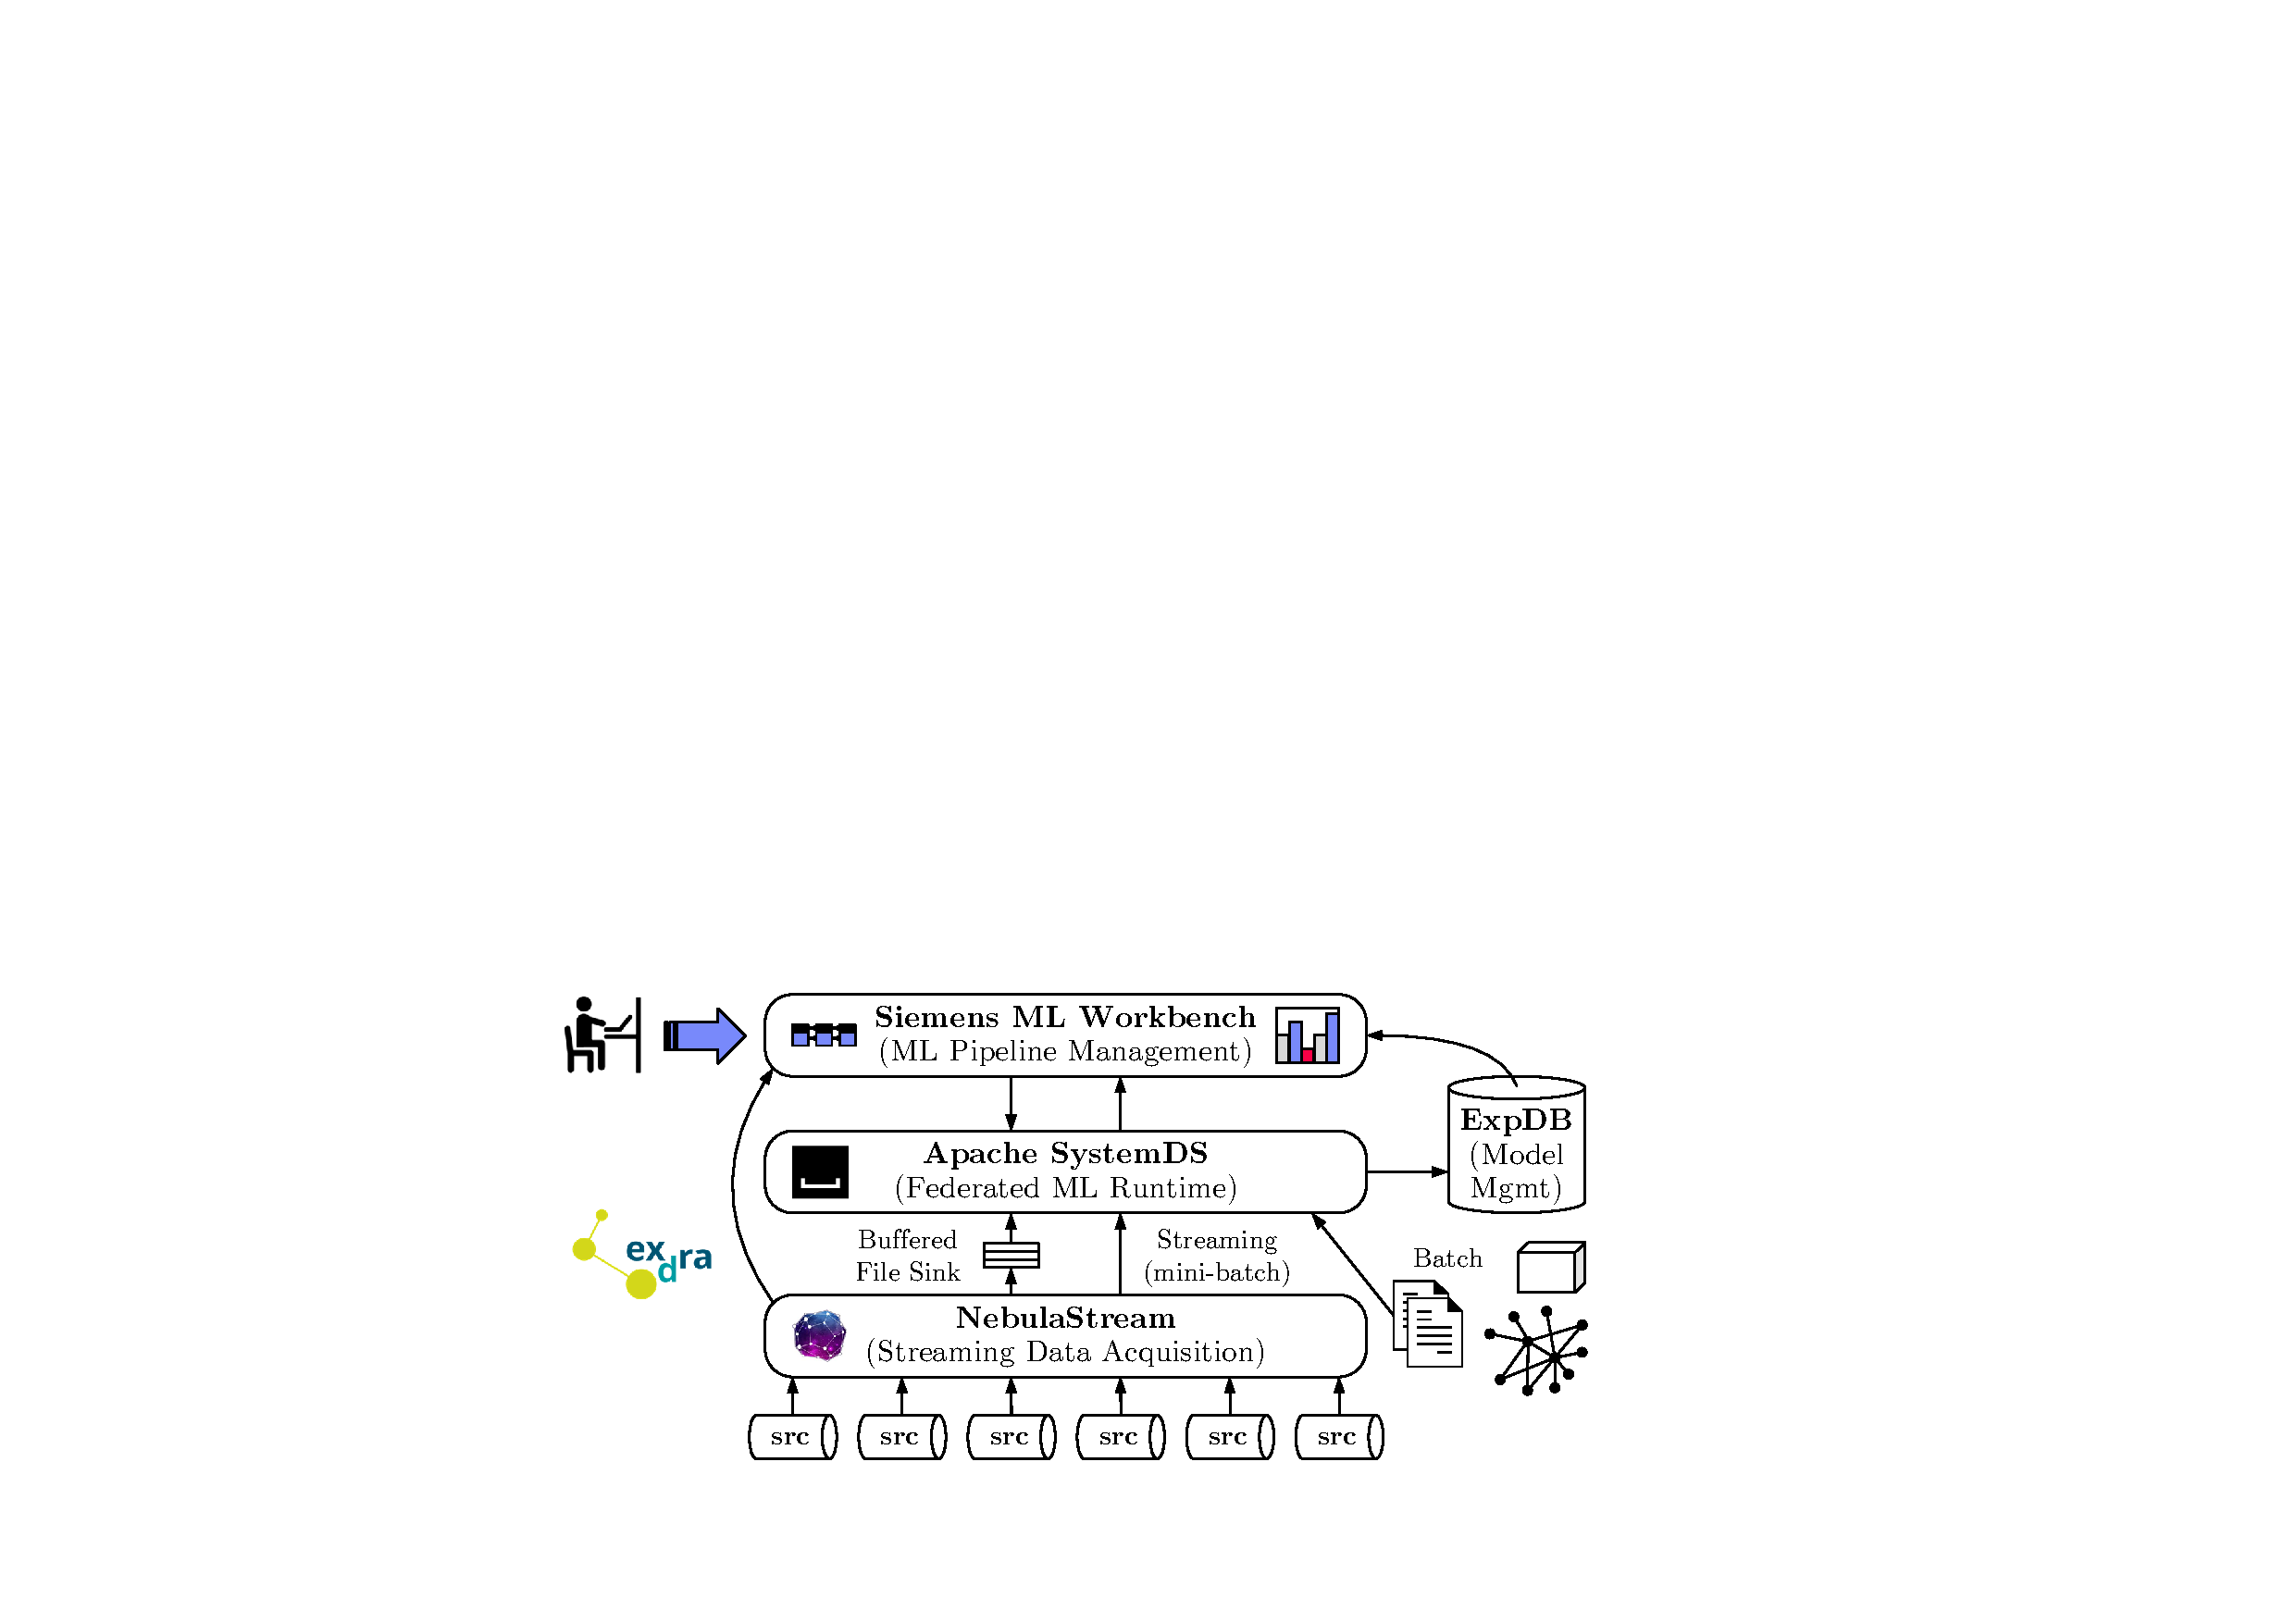
\includegraphics[scale=0.43]{figures/fig01}
	\vspace{-0.25cm}
	\caption{\label{fig:sysarch}ExDRa System Architecture.}
\end{figure}

\subsection{Workbench and Pipeline Management}
\label{sec:demo}

The UI is part of an ML workbench for project and pipeline management, developed by Siemens. Data scientists create and share projects, which contain data sources, ML pipelines, and interactive result plots. This pipeline management supports a variety of ML systems (e.g., Scikit-learn~\cite{PedregosaVGMTGBPWDVPCBPD11}, TensorFlow~\cite{AbadiBCCDDDGIIK16}, Apache MXNet~\cite{ChenLLLWWXXZZ15}, and pandas~\cite{mckinney-proc-scipy-2010}), and the system is designed for good scalability with increasing number of pipelines and users. 

\textbf{Frontend and Backend:} The frontend is based on the web framework Angular, and interfaces with a SpringBoot Java backend. Users compose ML pipelines of pre-defined data sources and pipeline steps (e.g., for pre-processing and ML algorithms), through the graphical UI. The backend stores configurations of data sources, pipeline steps, and pipelines. Supported data sources---which can be shared among pipelines---include text files like CSV, hierarchical binary data like HDF5, relational databases, object stores like AWS S3, and even message queues. Similarly, our ExperimentDB (for model analysis) and NES file sinks are integrated as data sources as well. The backend then triggers the execution of pipelines in so-called AI containers, and returns the results to the frontend.

\textbf{AI Containers:} The ML pipelines are executed in Docker containers on AWS ECS or Kubernetes \cite{BurnsGOBW16}. Each pipeline step is a Python script, and a dedicated container-local Java application (invisible to a user) connects to the central data sources, orchestrates the Python scripts according to the pipeline definition, and returns the results. Similar to the other ML systems, SystemDS and ExperimentDB are used through their respective Python APIs. 

\subsection{Federated ML Runtime}

In this infrastructure, SystemDS is used as federated runtime backend for ML algorithms and pipelines on raw data. For a seamless integration with common data science workflows and the ML workbench (Section~\ref{sec:demo}), SystemDS has been extended by a new Python API with lazy evaluation. Users create matrices or frames from federated configurations, files, NumPy arrays, or pandas data frames. The API further exposes operations and higher-level built-in functions, whose calls are collected in a DAG of operations. 

\small \vspace{0.1cm}
\begin{verbatim}
 features = Federated(sds, [node1,node2], ([…],[…]))
 model = features.l2svm(labels).compute()
\end{verbatim}
\normalsize \vspace{0.1cm}

\noindent On calling \texttt{compute}---similar to Dask~\cite{dask}---on an intermediate, we generate a DML script via depth-first DAG traversal for ordering according to data dependencies, execute this script, and return the result as a NumPy array or data frame. For federated learning, SystemDS supports both federated linear algebra, and federated parameter servers, which we discuss in detail in Section~\ref{sec:federated}. Instead of providing labor-intensive implementations of individual federated ML algorithms, this design aims to provide the necessary primitives such that a wide variety of built-in functions and ML algorithms can be automatically compiled into federated runtime plans.
 
\subsection{Model Management and Experiments}

Our ExperimentDB provides means of model and experiment management for exploratory data science. To this end, ExperimentDB comprises two major components:  a model and metric store, and a pipeline recommendation engine.

\textbf{Model Store:} We store trained models of pipeline versions (i.e., different artifacts), and their runs (i.e., with different parameters and input data). The inputs are the pipelines of AI containers (Section~\ref{sec:demo}), their output models, related accuracy metrics, and other metadata such as lineage and reusable intermediates. If a pipeline is marked for tracking, the workbench backend uses an ExperimentDB API to make these inputs available. The Python scripts are then parsed into an intermediate representation of a data flow graph, and individual pipeline steps are categorized accordingly. We use high-level operator types such as ensembles, estimators, imputers, scalers, selectors, generators, samplers, and transformers. This model store and collected metadata then allows for query-based pipeline comparisons, explanations, and analysis.
 
\textbf{Pipeline Recommendation:} Beyond basic model management, we further aim to provide (in the future) pipeline recommendations. Given a high-level ML task, dataset and its data characteristics, optional evaluation metric, and history of pipeline runs and their accuracy, the goal is to recommend a ranked list of pipelines for exploration. In contrast to AutoML, this process entails human-machine interaction for pipeline synthesis and debugging, as well as multi-model data analysis, which partially allow for self-supervision and thus, avoids the need for predefined metrics or labels. Our current prototype computes embeddings of pipeline metadata, and trains an ML model to predict scores of pipeline candidates.

\subsection{Streaming Data Acquisition}

Highly-distributed, potentially moving and unreliable, streaming data sources are a particularly challenging form of federated raw data. Exploratory data science and ML model training are repetitive and thus, require multiple passes over the data. We mitigate this impedance mismatch by leveraging NebulaStream (NES) for managing the low-level aspects of streaming data acquisition.

\textbf{NES Overview:} A central coordinator deploys continuous queries in a decentralized topology of heterogeneous nodes and devices. Inputs are sensor or consolidated logical streams. Operators of physical execution plans are then assigned and re-optimized \cite{GrulichBZTBCRM20} according to existing queries, available resources, utilization, and topology changes (e.g., moving robots/equipment). The node runtime receives and sends input and output streams, processes multi-threaded tasks, checks privacy constraints, triggers actuators, and provides inbound adapters like OPC (open platform communications) for integrating existing measurement systems.

\textbf{ExDRa Integration:} Within the ExDRa system infrastructure, separate NES instances---each with a coordinator and decentralized topology---get deployed at the individual federated sites, which protects private data by avoiding consolidation in central cloud environments. For exploratory use cases, NES appends the collected streams to file sinks with retention periods (e.g., last two days). ML pipelines then read this federated data from the file sink, and use an in-memory snapshot for iterative training. The file sinks and NES queries are deployed as federated data sources in the ML workbench (Section~\ref{sec:demo}). For deployment use cases, NES can also directly feed into the interactive visualization, and trigger mini-batch model updates for online learning. In the future, NES also aims to push down sink predicates, and other operations of deployed ML pipelines, into the continuous queries.

%%%%%%%%%%%%%%%%%%%%%%%%%%%%%%%%%%%%%%%%%%%%%%%%%%%%%%%%%%%%%%%%%%%%%%%%%%%%%%%%%%%%%%%%%%%%%%%%%%%%
\section{Federated Runtime}
\label{sec:federated}

Apache SystemDS \cite{BoehmADGIKLPR20} supports multiple runtime backends for local, in-memory operations (CPU/GPU), and distributed operations on Apache Spark \cite{ZahariaCDDMMFSS12}. The new federated backend\footnote{The entire federated runtime backend is available open source as part of Apache SystemDS: \url{https://github.com/apache/systemds}.} follows a similar design of specific federated data objects, and runtime instructions. Here, we describe the overall design, federated linear algebra operations, federated parameter servers, federated data preparation, and our vision for federated ML pipelines on raw data. 

\subsection{Federated Data and Backend Design}
\label{sec:design}

SystemDS compiles user scripts of ML algorithms or pipelines into hybrid runtime programs of local and distributed operations. A main control program (CP)---potentially in the Spark driver---then executes the control flow and operations as instructions. Live variables are accessible via a symbol table. Figure~\ref{fig:federated} shows this setup and the integration of the federated backend.

\begin{figure}[!t]
	\centering
	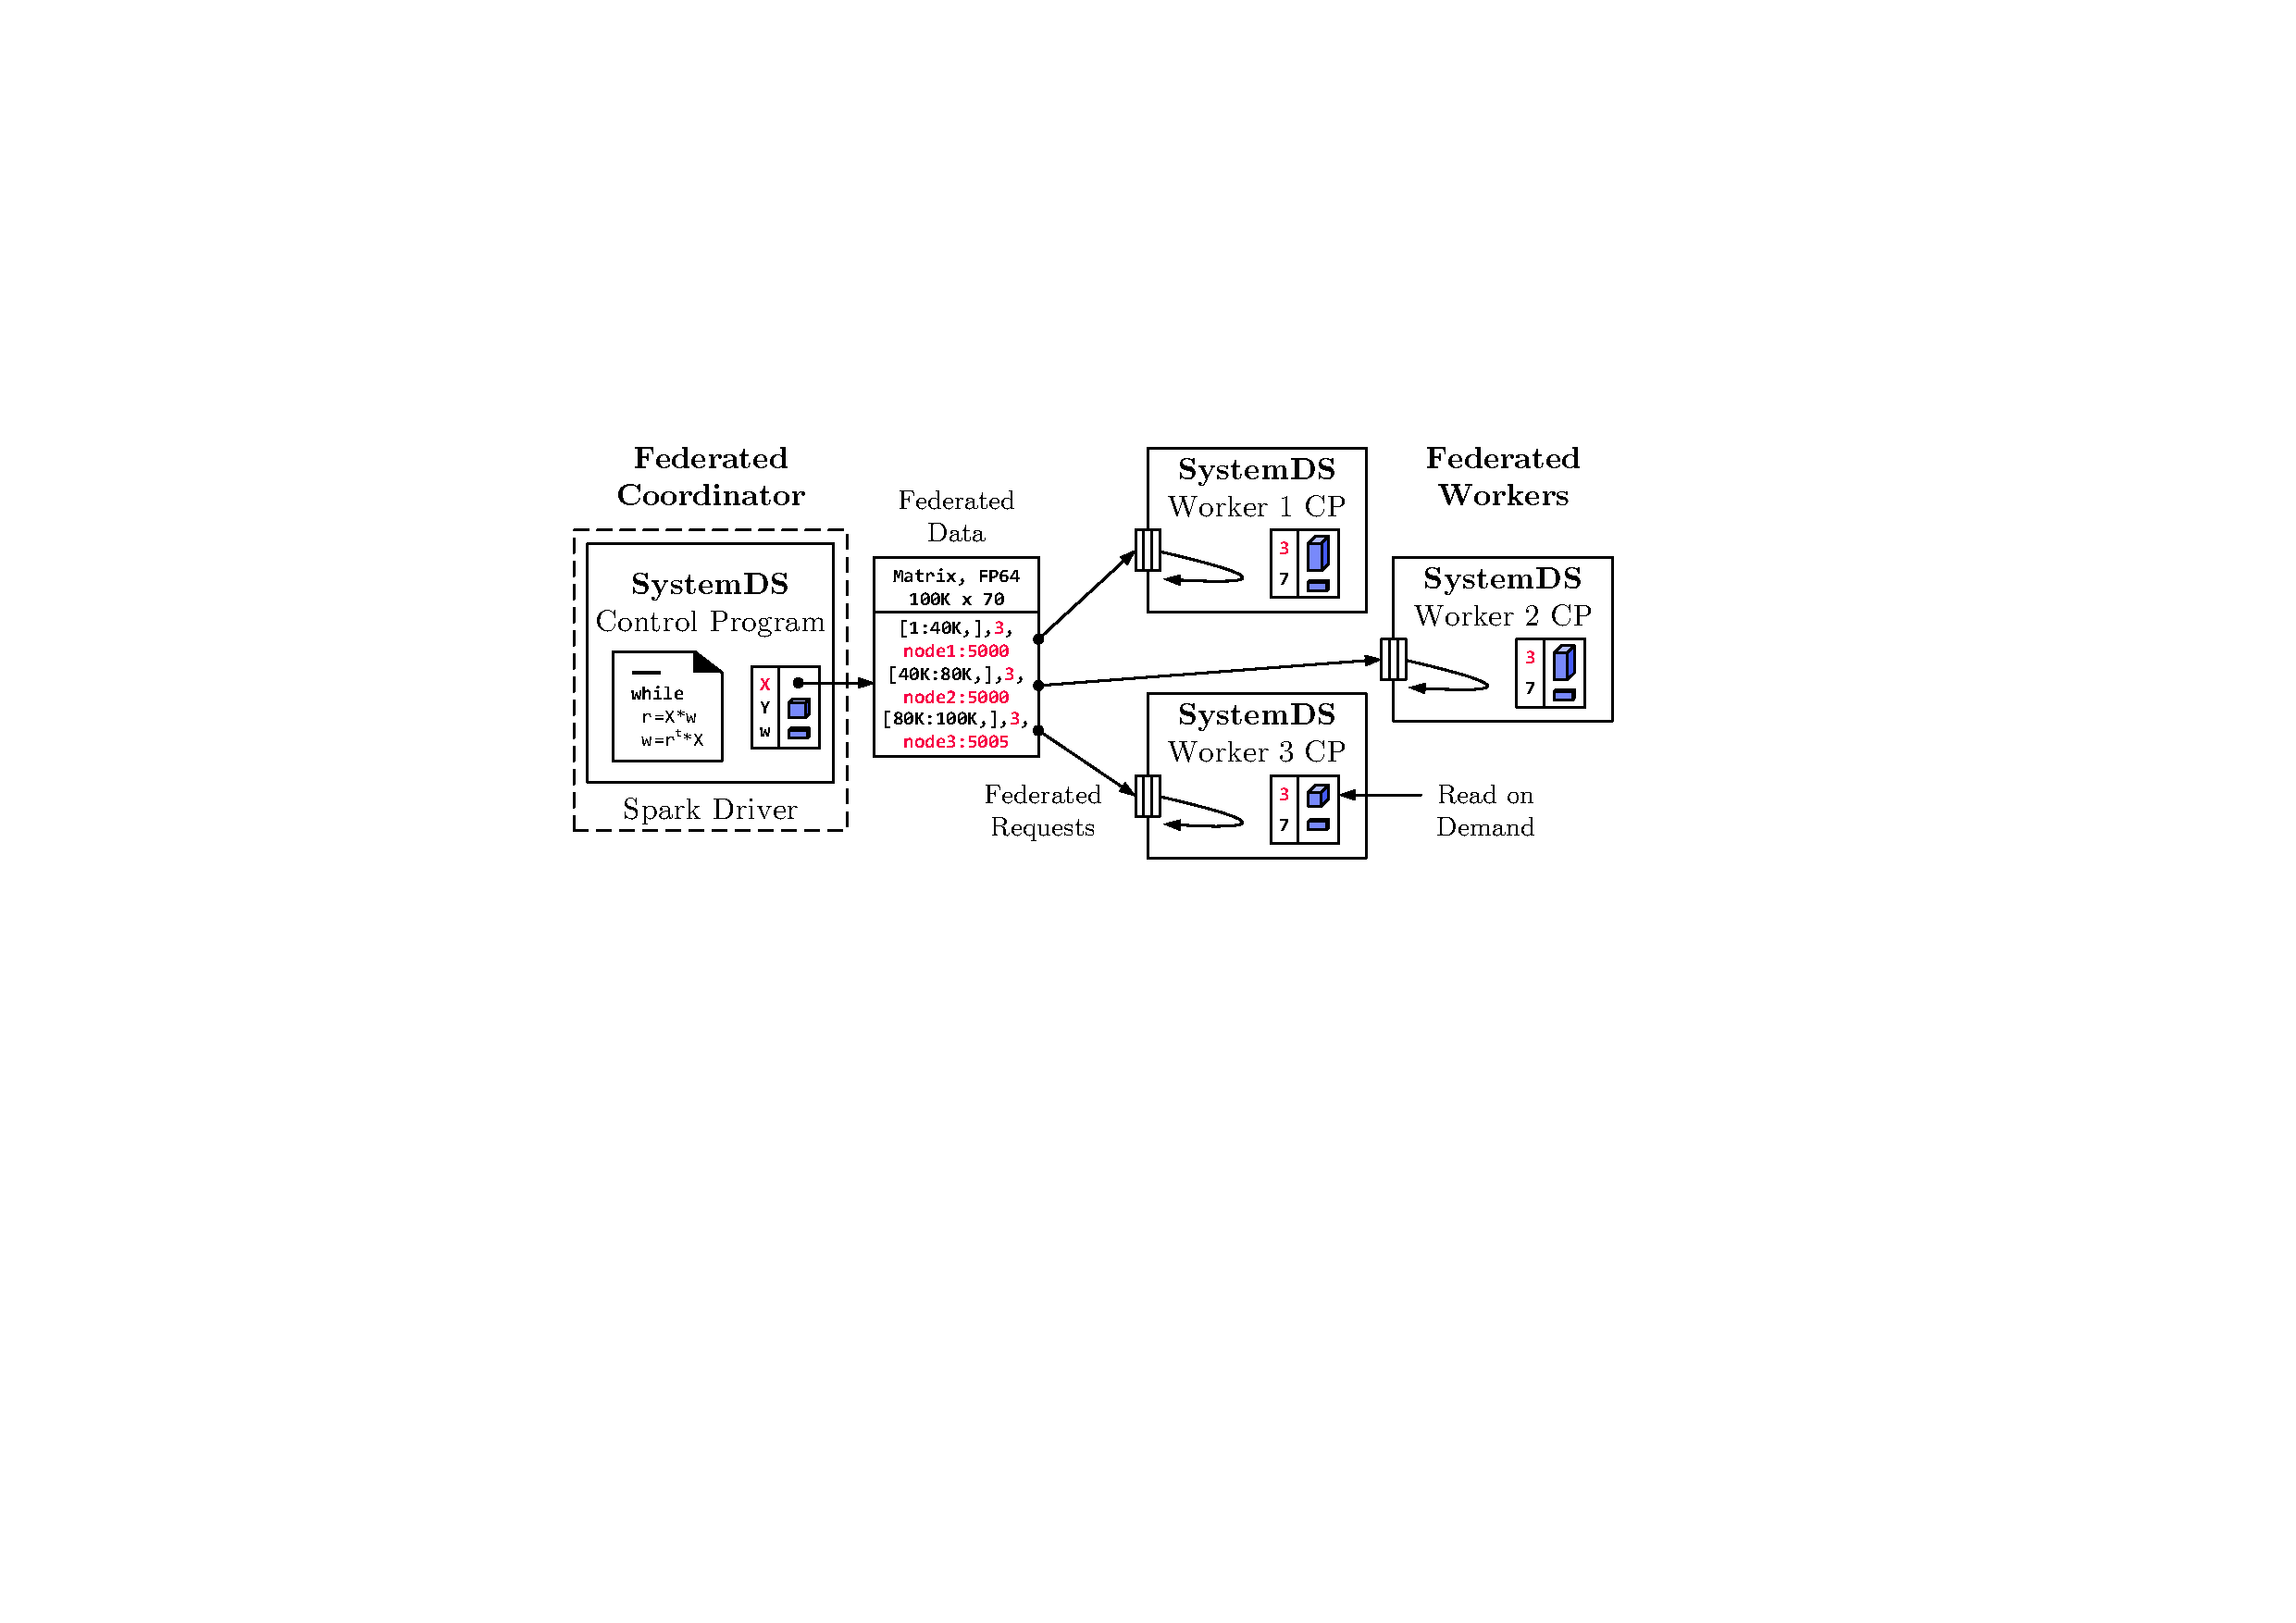
\includegraphics[scale=0.43]{figures/fig02}
	\vspace{-0.25cm}
	\caption{\label{fig:federated}Federated Runtime Backend.}
\end{figure}

\textbf{Federated Data:} Any non-scalar data objects such as tensors, matrices, and frames can be federated. The main control program acts as the coordinator and holds only metadata---in the form of a federation map---of such federated data. This map stores the data type, value type, dimensions,  sparsity, as well as non-overlapping data ranges, and their locations (host, port, data identifier). For example, in Figure~\ref{fig:federated}, we have a federated $100\text{K} \times 70$ matrix $\mat{X}$, with row partitions $[1{\,:\,}\text{40K}]$, $[\text{40K}{\,:\,}\text{80K}]$, and $[\text{80K}{\,:\,}\text{100K}]$ on node1, node2, and node3, respectively. If a local operation at the coordinator tries to pin $\mat{X}$ into memory, the federated data is transparently transferred---unless it violates coarse-grained or fine-grained privacy constraints---and consolidated in a local matrix.

\textbf{Federated Workers:} Similar to the coordinator, the federated workers are also control programs, but started as worker processes that act like servers at the federated sites. A worker listens on an input queue for incoming RPC requests (called federated requests), executes these requests, maintains a local symbol table, checks privacy constraints (e.g., for data exchange), and finally returns an---optionally SSL-encrypted---RPC response. This design of worker CP programs provides very good flexibility and reuses the I/O subsystem, buffer pool mechanisms, as well as local and distributed operations. For example, it even allows data center federation \cite{VulimiriCGKV15}, where a single federated operation triggers distributed operations in a Spark \cite{ZahariaCDDMMFSS12} or Flink \cite{AlexandrovBEFHHKLLMNPRSSHTW14} cluster at the federated site.

\textbf{Federated Requests:} The coordinator communicates with workers through federated requests, using Netty as a network I/O framework for RPCs and data transfers. To simplify the implementation of federated operations, we restricted the federation protocol to only six generic request types:
\begin{itemize2}
\item \texttt{READ(ID, fname)}: Creates a data object from a filename, reads it, and adds it by ID to the symbol table.
\item \texttt{PUT(ID, data)}: Receives a transferred data object, and adds it by given ID to the symbol table. 
\item \texttt{GET(ID)}: Obtains a data object from the federated site's symbol table, and returns it to the coordinator.
\item \texttt{EXEC\_INST(inst)}: Executes an instruction, which accesses inputs and outputs by IDs in the symbol table.
\item \texttt{EXEC\_UDF(udf)}: Receives a serialized, user-defined function (UDF) object, executes this UDF over requested inputs by ID, may add outputs to 
the symbol table, and returns a custom object to the coordinator.
\item \texttt{CLEAR}: Cleans up execution contexts and variables.
\end{itemize2}
For efficiency, the coordinator sends RPCs to all workers in parallel, and a single RPC can contain a sequence of requests and returns a single response. The simplicity of these request types has two profound advantages. First, we can reuse existing instructions for composing federated operations. Second, this design allows for federation hierarchies. If the worker-local data is federated data, a worker can also act as a coordinator of a subgroup of workers.

\subsection{Federated Linear Algebra}

For broad applicability in various ML algorithms and data science lifecycle tasks, our federated runtime supports both federated linear algebra and federated parameter servers. Federated linear algebra utilizes similar strategies as distributed, data-parallel operations but retains the raw federated data at its federated site. This requirement creates additional challenges and needs compiler support for finding valid yet efficient runtime plans if operations do not directly apply.

\textbf{Basic Linear Algebra:} During compilation and runtime, we check if any inputs are federated data, and dispatch this call to supported federated instructions. Similar to RDD transformations and actions \cite{ZahariaCDDMMFSS12}, these federated instructions then utilize federated requests---and related high-level primitives for broadcasting and aggregation---to compute the operations over federated data. If no aggregation is needed, the output is itself federated data. 

\begin{example}[Federated Matrix Multiplication]
Assume a matrix-vector (or matrix-matrix with small right-hand-side) multiplication $\mat{X}\,\mat{v}$ and vector-matrix multiplication $\mat{v}^{\top}\,\mat{X}$ with $\text{nrow}(\mat{X}) \gg \text{ncol}(\mat{X})$ and $\mat{X}$ being composed of federated row partitions. For matrix-vector, we broadcast $\mat{v}$ via \texttt{PUT}, execute a local matrix-vector multiplication per partition via \texttt{EXEC\_INST}, which yields a new federated vector with related federation map (logical \texttt{rbind} here), and finally execute an optional \texttt{rmvar} instruction via \texttt{EXEC\_INST} to clean up the broadcast $\mat{v}$. In contrast, for a vector-matrix, we perform a sliced broadcast of $\mat{v}$ (vector parts according to row ranges), execute a local vector-matrix multiplication per partition via \texttt{EXEC\_INST}, obtain the results via \texttt{GET}, do a final aggregation via element-wise vector addition at the coordinator, and again, clean up all intermediates. 
\end{example}


\begin{table}[!b]
\centering \small \setlength\tabcolsep{7pt}
  \caption{\label{tab:inst}Example Federated Instructions.}
	\vspace{-0.4cm}
  \begin{tabular}{cc}
	  \toprule
		\textbf{Operation Type} & \textbf{Examples}\\
		\midrule
    Matmult & \texttt{mm}, \texttt{tsmm}, \texttt{mmchain}\\
		Aggregates & \texttt{sum}, \texttt{min}, \texttt{max}, \texttt{sd}, \texttt{var}, \texttt{mean}\\
		        & \texttt{rowSums}, \ldots, \texttt{rowMeans}, \texttt{colSums}, \ldots, \texttt{colMeans}\\
		Unary & \texttt{abs}, \texttt{cos}, \texttt{exp}, \texttt{floor}, \texttt{isNA}, \texttt{log}, \texttt{!}, \texttt{round}, \texttt{sin},\\
		      & \texttt{sign}, \texttt{softmax}, \texttt{sqrt}, \texttt{tan}, \texttt{sigmoid},\\
		Binary & \texttt{\&}, \texttt{cov}, \texttt{cm} \texttt{/}, \texttt{=}, \texttt{>}, \texttt{>=}, \texttt{\%/\%}, \texttt{<}, \texttt{<=}, \texttt{log},\\
		& \texttt{max}, \texttt{min}, \texttt{max}, \texttt{-}, \texttt{\%\%}, \texttt{*}, \texttt{!=}, \texttt{|}, \texttt{+}, \texttt{\^}, \texttt{xor}\\
		Ternary & \texttt{ctable}, \texttt{ifelse}, \texttt{+*}, \texttt{-*} \\
		Quaternary & \texttt{wcemm}, \texttt{wdivmm}, \texttt{wsigmoid}, \texttt{wsloss}\\ 
		Transform/Reorg & \texttt{tfencode}, \texttt{tfapply}, \texttt{tfdecode}, \\
		                & \texttt{rbind}, \texttt{cbind}, \texttt{t} (transpose), \texttt{removeEmpty}\\
										& \texttt{replace}, \texttt{reshape}, \texttt{X[:,:]} (matrix indexing)\\
		\bottomrule
	\end{tabular}
	\normalsize
\end{table}


\textbf{Supported Operations:} So far, we support---as summarized in Table~\ref{tab:inst}---federated matrix multiplication, unary aggregates, unary element-wise operations, binary matrix-matrix, matrix-vector, and matrix-scalar operations, ternary, quaternary, and parameterized builtin operations, and various reorganizations. These operations further support both row- and column-partitioned federated data via specialized implementations. Most of the binary operations (e.g., matmult, element-wise) support a single federated input and consolidate a second federated input (e.g., aggregated intermediates) in the coordinator. However, whenever two federated inputs are co-partitioned (e.g., because one originated from the other), we directly execute federated operations on them as well. 

\textbf{Higher-level Primitives:} SystemDS follows the premise that many data science lifecycle tasks---like data validation, data cleaning, feature and model selection, and model debugging---are themselves based on machine learning and numerical computation \cite{BoehmADGIKLPR20}. These higher-level primitives are hierarchically composed from built-in functions that rely on linear algebra and thus, are directly supported on federated data as well. In case a binary or ternary operation is not supported over multiple federated matrices, some of them are consolidated in the coordinator, or a privacy exception is thrown if this consolidation would reveal private raw data. For this reason, we are working toward better compiler support that proactively considers privacy constraints and generates efficient runtime plans that adhere to these constraints. 

\begin{example}[Federated K-Means] \label{ex:kmeans}
Starting bottom-up, individual ML algorithms are good examples of such higher-level primitives. For instance, consider the inner loop (after initialization and inside a loop for multiple runs) of K-Means clustering, where $\mat{X}$ is a federated, row-partitioned matrix, and $\mat{C}$ are the current centroids:

\small \vspace{0.1cm}
\begin{verbatim}
 while (term_code == 0) {
   # Compute Euclidean squared distances records-centroids   
   D = -2 * (X %*% t(C)) + t(rowSums(C ^ 2));
   # Find the closest centroid for each record
   P = (D <= rowMins(D));
   # If records belong to multiple centroids, share them
   P = P / rowSums(P);
   # Compute the column normalization factor for P
   P_denom = colSums(P);
   # Compute new centroids as weighted averages
   C_new = (t(P) %*% X) / t(P_denom); # ...
 }
\end{verbatim}
\normalsize \vspace{0.1cm}

\noindent The first matrix multiplication $\mat{X}\, \mat{C}^{\top}$ yields another federated, row-partitioned matrix. The subsequent row aggregates and element-wise operations similarly create aligned federated intermediates, which are then aggregated and only consolidated in aggregate form via $\text{colSums}(\mat{P})$ and $\mat{P}^{\top}\, \mat{X}$, where the latter is an aligned matrix multiplication of two federated matrices. Note that this built-in function script is agnostic of local, distributed, or federated input matrices.
\end{example}

While some ML algorithms directly map to federated operations that preserve private data, other algorithms need dedicated compiler assistance for generating valid runtime plans. Specifying data exchange (i.e., privacy) constraints for federated raw data, tracking derived properties of intermediates and data transfers, and generating constraint-aware plans is an important direction for future work but beyond the scope of this paper.

\subsection{Federated Parameter Server}
\label{sec:paramserv}

The federated linear algebra backend described so far supports traditional batch ML algorithms (e.g., first- and second-order) as well as high-level primitives, but would be very inefficient for mini-batch algorithms---as used for DNNs---because most federated workers would stay idle while processing a batch at-a-time. Such mini-batch algorithms are usually trained with data-parallel parameter servers or similar distribution strategies. Accordingly, we  extended SystemDS' parameter server (PS) for federated data as well.

\textbf{Background SystemDS PS:} The existing SystemDS PS infrastructure implements a traditional, data-parallel parameter server \cite{SmolaN10,DeanCMCDLMRSTYN12,LiAPSAJLSS14,JiangCZY17}, where a central server maintains the current model, and workers pull the model, perform mini-batch iterations over disjoint data partitions to compute gradients, and push these back to the server for aggregation. This functionality is integrated as a native built-in function and can be invoked in a stateless manner: 

\small \vspace{0.1cm}
\begin{verbatim}
 M = list(W1, W2, W3, W4, b1, b2, b3, b4, ... vW4); # model
 params = list(lr=lr, mu=mu, stride=stride, pad=pad, ...);
 Mp = paramserv(model=M, features=X, labels=y, 
                upd=updateGrad, agg=updateModel, utype=ASP,
                freq=BATCH, epochs=200, batchsize=64, ...);
\end{verbatim}
\normalsize \vspace{0.1cm}

\noindent The initialized model---as a list of weight and bias matrices, as well as additional state matrices like the parameter velocities---and data is passed as arguments, along with a configuration of update types (e.g., BSP -- bulk-synchronous parallel, ASP -- asynchronous), update frequencies, batch size, number of epochs, data partitioner, hyper-parameters, and user-defined functions for computing gradients (\texttt{updateGrad}), updating the model with gradients (\texttt{updateModel}), and optional validation. Internally, the parameter server then either runs in local, multi-threaded or distributed Spark mode, where the latter runs the parameter server locally at the coordinator, spawns a Spark job with standing worker tasks and directly communicates via RPCs between the parameter server and workers.

\textbf{System Architecture:} The federated parameter server exhibits a similar PS architecture, consisting of a server running at the coordinator, and workers at the federated sites for computing gradients on the private data. During setup, we serialize the gradient and update functions and send them to the workers. Then one server thread per worker handles the communication and synchronization with federated workers, which are executed via a \texttt{EXEC\_UDF(udf)} federated request. Depending on the updated frequency, the model is updated at the worker, and after a fixed number of batches, the accrued gradients are sent to the server for aggregation. In contrast to SystemDS' multi-threaded parameter server, the gradient function is compiled in a way that leverages multi-threaded operations with the available degree of parallelism at each worker.

\textbf{Federated Data Partitioning:} In a typical PS architecture, the input data is potentially shuffled for randomization, and then evenly partitioned horizontally among workers. In contrast, the federated parameter server respects the locality of federated data (specifically, row-partitioned and aligned federated data $\mat{X}$ and labels $\mat{y}$), which allows only local shuffling and replication of the private federated data. The chosen partitioning strategy---unless the data is used without modification---is again executed via a \texttt{EXEC\_UDF(udf)} federated request before the start of iterative training. 


\begin{figure*}[!t]
	\centering
	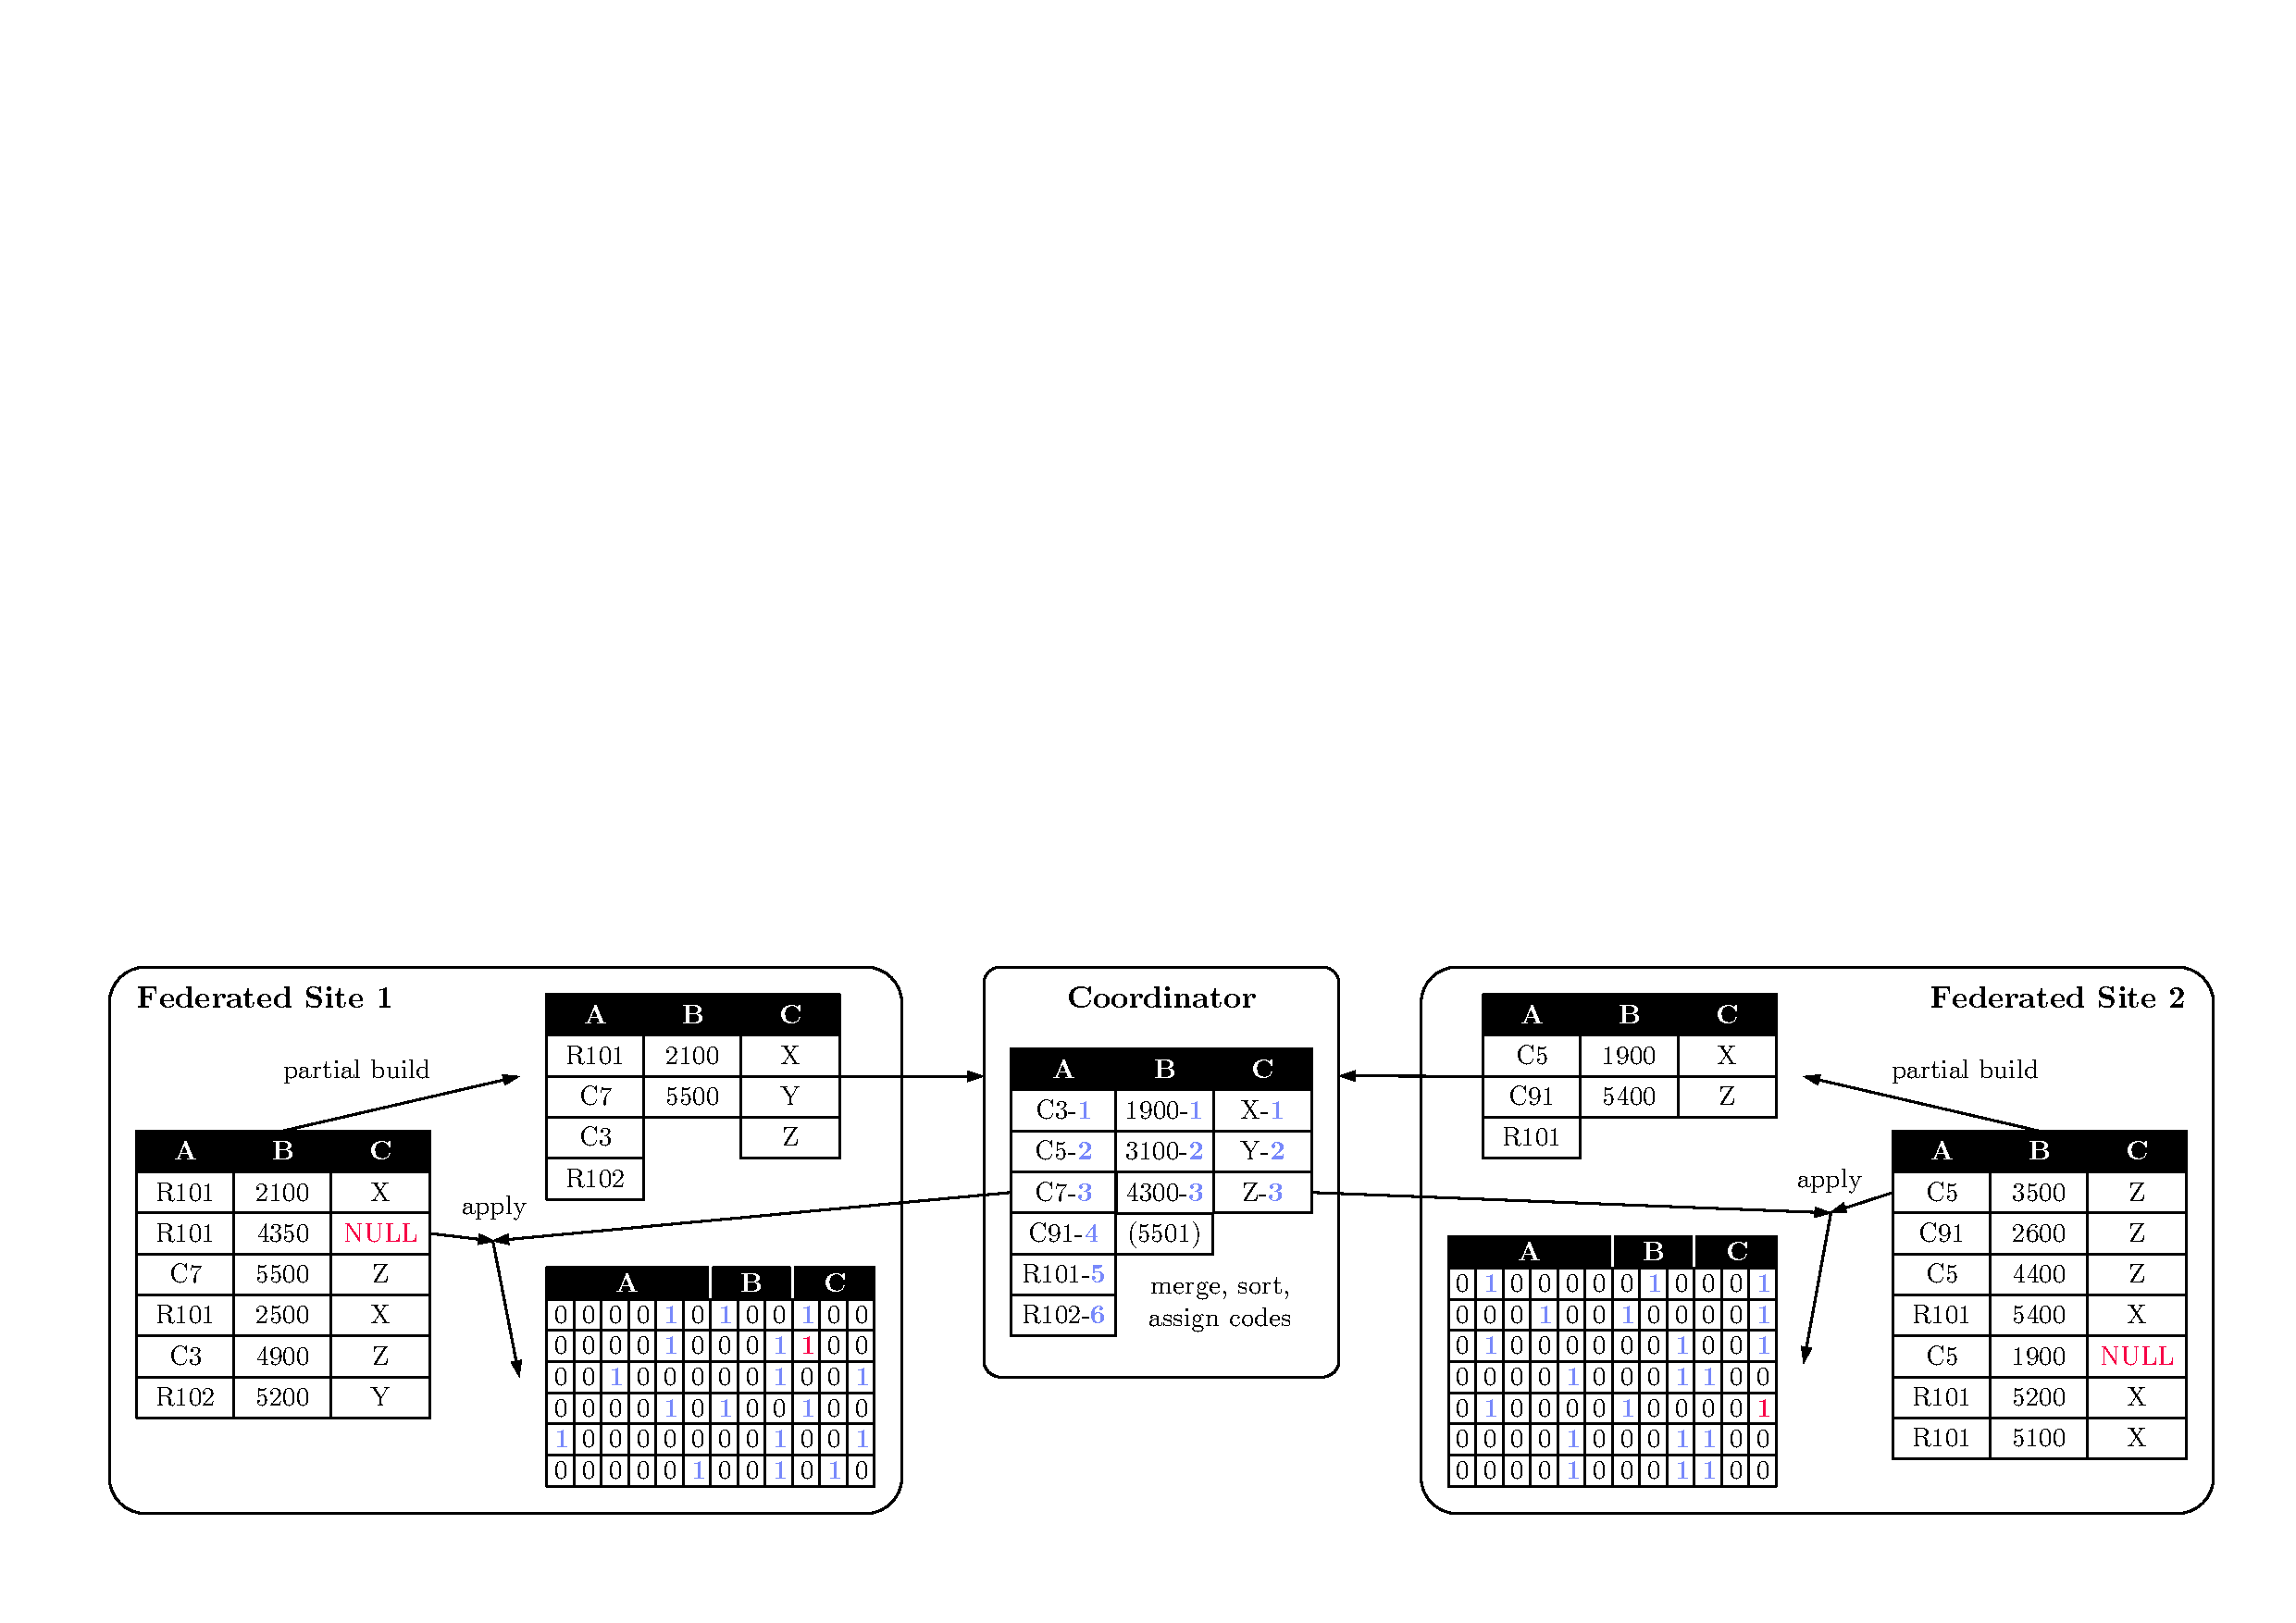
\includegraphics[scale=0.43]{figures/fig03}
	\vspace{-0.25cm}
	\caption{\label{fig:transform}Example Federated Transformencode (binning, recoding, and one-hot encoding).}
	\vspace{-0.15cm}
\end{figure*}


\textbf{Handling Imbalance and Skew:} A major challenge in the federated setting is the handling of imbalance in terms of different worker data sizes, and skew of the data distributions at the different federated workers. Imbalance and skew (also known as statistical heterogeneity \cite{LiSTS20,Smith20}) are problematic because an equal number of epochs results in different numbers of iterations and thus, skew in execution time, coordination problems in synchronous update strategies like BSP (where the parameter server waits for all worker updates), and biased updates, where the biggest federated data partition solely influences model updates at the end of training. Subsampling large or replicating small partitions on the other hand puts disproportionate weight on the observations of small federated partitions. We are currently using replication with adjusted weights, but subsampling and replication, weighting schemes, and hierarchical parameter server architectures (similar to virtual nodes in Dynamo \cite{DeCandiaHJKLPSVV07}) is a rich area for future work.

\subsection{Federated Data Preparation}
\label{sec:dataprep}

Besides ML-based data cleaning and data pre-processing---which are based on federated linear algebra---there are other data preparation techniques that require special federated support. These operations include feature transformations, and data access methods for raw data. In contrast to typically stateless ML systems and libraries, the architecture of standing federated workers further provides rich opportunities for reuse and adaptive data reorganization across multiple pipeline runs of a single user and multiple tenants.

\textbf{Feature Transformations:} Similar to other, commonly-used ML systems, SystemDS supports---through operations like frame \texttt{transformencode} and \texttt{transformapply}---standard feature transformations like recoding (categories to integers), feature hashing (categories to upper-bounded integers, potentially with collisions), binning (numeric values to integers), and one-hot encoding (integers to sparse boolean vectors). The federated instructions of these operations leverage the flexibility of UDFs via \texttt{EXEC\_UDF} and preserve privacy of the raw federated data. In detail, federated \texttt{transformencode} uses a two-pass approach. First, we build encoder-specific metadata for all non-pass-through features (i.e., all columns except unmodified numeric columns) at the federated sites, as well as consolidate---and optionally sort---the metadata for consistent encoding. Second, we broadcast the aggregated metadata, and in a second pass over the federated data, then perform the actual encoding. The outputs are a federated encoded matrix with consistently aligned one-hot encoded features (equivalent to local encoding), and a local metadata frame.

\begin{example}[Federated One-hot Encoding]
Figure~\ref{fig:transform} shows an example of a row-partitioned federated input frame with three columns A, B, and C. Here, A and C are categorical features subject to recoding and one-hot encoding, while B is a numerical feature subject to binning (with three equi-width bins) and one-hot encoding. Not all categories will appear in all federated sites. For example, feature A represents regular and custom recipes of our paper production use case from Section~\ref{sec:paper}. In a first step, the federated workers compute the distinct items for recoded features and min/max values for binned features. The coordinator consolidates these metadata frames from the federated sites, merges and sorts the distinct items, computes the bin boundaries, and finally assigns contiguous integer codes. In a second step, the global metadata is sent to the federated sites for encoding the input frame into a numeric matrix. Non-existing categories lead to all-zero columns but this encoding ensures consistent feature positions for model training. Federated linear algebra then further allows applying various techniques for data cleaning and missing value imputation. These primitives are implemented as script-based built-in functions and thus, can now be compiled into federated runtime plans as well. For instance, the NULLs (or NAs) in column C might be imputed with the mode (most frequent categorical value, imputing \texttt{X} or \texttt{Z}), via robust functional dependencies \cite{DengFAWSEIMO017} (assuming or discovering $A \rightarrow C$, and imputing \texttt{X} and \texttt{Z}, respectively), or by more advanced, ML-based techniques like multivariate imputation by chained equations (MICE, which trains regression and classification models for imputing categorical and numerical columns) \cite{JSSv045i03,CambroneroFSM17}. 
\end{example}

\textbf{Improved Feature Transformations:} There are many opportunities for improved federated feature transformations. First, techniques like zigzag joins \cite{TianOZGP16}---that rely on Bloom filters for pre-filtering---can be adapted for determining categories that need to be exchanged with the coordinator, thereby reducing data transfer and revealed information. Similarly, for features that only exist at a single federated site (e.g., column-partitioned federated data), we only need to exchange the number (instead of the set) of distinct items. Second, there is a tradeoff between privacy and performance versus accuracy. Instead of recoding, users can resort to feature hashing (with an agreed hash function), which is computed in a purely federated manner without data exchange. However, hash collisions merge multiple categories into one feature, which might negatively affect accuracy. In our current implementation we support the different transformations but leave the choice up to the user because we expect related negotiations among involved parties.

\textbf{ML Pipelines on Raw Data:} The federated raw data is read as frames or heterogeneous tensors \cite{BoehmADGIKLPR20} into the standing workers and then accessed with federated indexing (e.g., for feature selection) and feature transformations (e.g., \texttt{transformencode}). Similar to low-latency scoring services, we already reuse deserialized recode maps at a fine granularity of individual features. Inspired by query processing on raw data \cite{AlagiannisBBIA12,IdreosAJA11,KarpathiotakisA16}, data reorganization via database cracking \cite{IdreosKM07} / adaptive indexing \cite{IdreosMG12}, recycling of intermediates \cite{IvanovaKNG10}, and lazy maintenance of materialized views \cite{ZhouLE07}, we further aim to leverage the opportunity of standing workers for adaptive data reorganization. Future work includes three main directions.
\begin{itemize}
\item \emph{Lineage-based Reuse:} First, we will establish lineage-based caches for reuse \cite{XinMLMSP18,DerakhshanMARM20} and debugging \cite{VartakTMZ18} of intermediates. As a first step, we have already integrated our LIMA framework for fine-grained lineage tracing and reuse \cite{LIMA21}. In this context, there is also potential for multi-tenant data structures that share partial overlap of feature subsets.
\item \emph{Compression:} Second, free cycles of federated workers can be used for asynchronous, lossless compression \cite{ElgoharyBHRR18,LiCZ00NP19} such as compression planning and compaction of intermediates.
\item \emph{Incremental Maintenance:} Third, the cached and reorganized intermediates can be---in case of applicable operations---incrementally maintained \cite{NikolicEK14,Schelter20} for new or deleted data.
\end{itemize}
In the context of exploratory ML pipelines with repeated raw data access and data enrichment, such a systematic reorganization would allow to eliminate unnecessary redundancy, and specialize the data representation for the observed workload characteristics, while retaining the appearance of a stateless ML system and preserving the privacy of the federated raw input data.


%%%%%%%%%%%%%%%%%%%%%%%%%%%%%%%%%%%%%%%%%%%%%%%%%%%%%%%%%%%%%%%%%%%%%%%%%%%%%%%%%%%%%%%%%%%%%%%%%%%%
\section{Towards Deployment in Production}
\label{sec:deployment}

The ExDRa infrastructure is \emph{not} deployed in production yet. However, the use cases described in Section~\ref{sec:usecases} are real production use cases, which exhibit potential for enterprise federated learning. In this section, we discuss in more detail the envisioned deployment of the ExDRa infrastructure, and other deployment models.

\subsection{Envisioned Deployment: Private Data}
\label{sec:basicdeploy}

SystemDS and NebulaStream are both large system projects, developed independently for different use cases of the end-to-end data science lifecycle and streaming IoT data management. For enterprise federated learning in the ExDRa infrastructure, both systems are jointly extended and their strengths come to bear in the envisioned deployment model. Most importantly, this setup enables us to mitigate the impedance mismatch between streaming data sources and iterative, multi-pass federated learning.

\textbf{Basic Deployment:} Figure~\ref{fig:deployment} shows the basic deployment model of enterprise federated ML in ExDRa. We assume a moderate number of federated sites (recently called cross-silo federated learning \cite{Smith20}), each with their local infrastructure and private raw data. At each federated site, a SystemDS worker is started as a standing server process, receiving federated requests from the coordinator via secure communication channels, and accessing permissioned raw data. Each site also deploys a NES instance with a coordinator and decentralized topology of workers and sensors for streaming data acquisition through distributed continuous queries (which are pre-configured but there is potential for partial push-down of deployed scoring pipelines). For training, NES appends the collected data to file sinks with configured retention periods, and every SystemDS ML training session reads the data, and works on a consistent in-memory snapshot. Thus, batch data and buffered streams are handled the same, which bridges the gap to iterative ML training. This execution model has well-defined semantics but long training sessions might work on partially stale data.

\textbf{Extensions for Stream Ingestion:} In contrast to the generic basic deployment, there are more specialized scenarios that allow ingesting input streams into SystemDS workers as well. First, federated parameter servers (see Section~\ref{sec:paramserv}) process the data in epochs, one batch of rows at a time. Here, the federated workers can seamlessly handle the removal or append of new batches according to the configured retention periods. However, changing data sizes require coordination to obtain imbalance ratios for replication and weight adjustments. Second, for deployed scoring pipelines SystemDS can act as a serving platform, processing the input streams and returning the predictions to the federated site or coordinator.  

\textbf{The Missing Pieces:} For deployment in production several challenges remain. First, from an organizational perspective, appropriate legal frameworks and business models need to be devised. Enterprise federated learning can be a win-win for large and small companies alike: large companies might run the infrastructure and model training; small and medium-sized enterprise (SMEs) may participate as federated sites, which opens up new income channels. In contrast to existing data marketplaces \cite{FruhwirthRP20}, participating federated sites can contribute to global model training without sharing their precious raw data. A crucial aspect is finding the right incentives for motivating the federated sites to participate with high-quality raw data (e.g., Jordan's leave-one-out proposal \cite{sysml}, or contractual benefits). Second, from a technical perspective, deployment in production requires a trusted system infrastructure, and techniques for generating and verifying federated execution plans under awareness of privacy constraints. Third, it is a never-ending quest for added business value, stronger privacy, and higher performance.

\begin{figure}[!t]
	\centering
	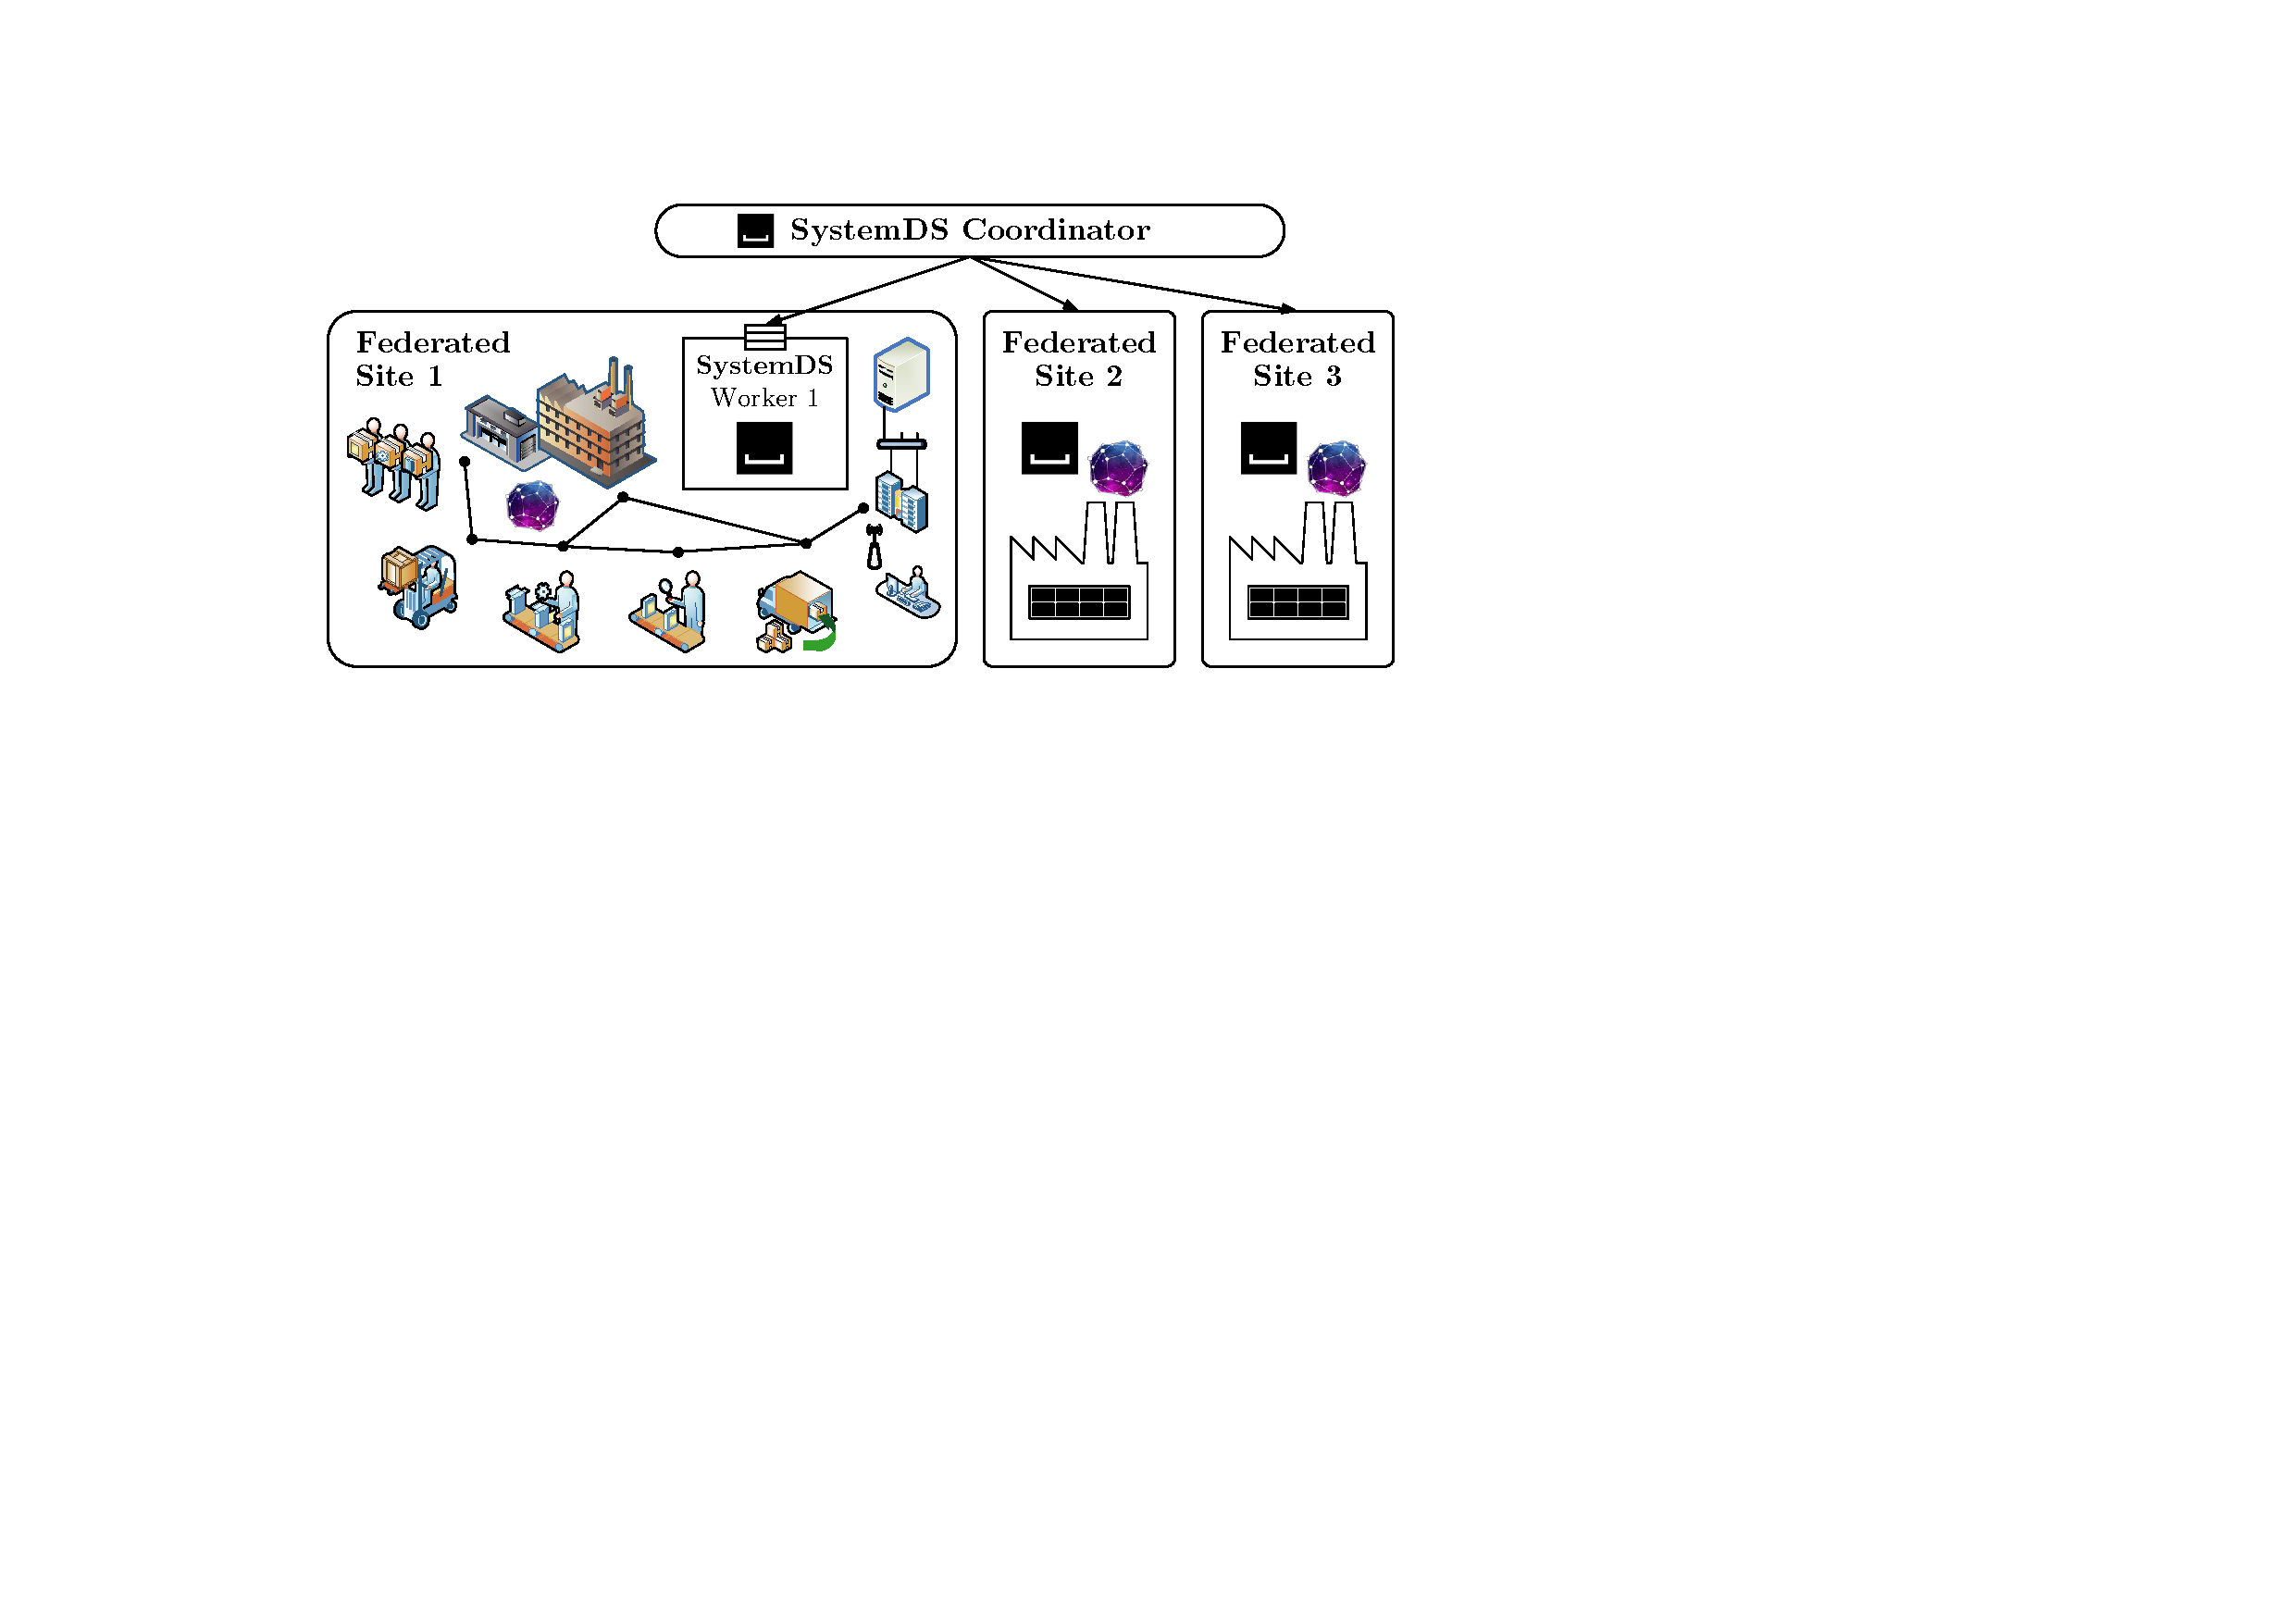
\includegraphics[scale=0.42]{figures/fig04}
	\vspace{-0.25cm}
	\caption{\label{fig:deployment}Envisioned SystemDS and NES Deployment.}
\end{figure}

\subsection{Other Deployments: Private Models}

Beyond our envisioned deployment for private federated data, there are other interesting deployments where federated ML models instead of federated data are kept private. For example, consider a scenario of a subsidiary company that receives---potentially anonymized---data from the parent company in order to derive predictions or create insights. Here, the ML models are the subsidiary's core assets. 
%KAI, Merkur Labs + Numerai
Similar examples include telecom providers sharing mobility data with partners for deriving insights, and hedge funds sharing financial data and predicting the stock market based on a stake-weighted federated ensemble of private models \cite{numerai}. Like enterprise federated ML, sharing only predictions prevents reverse-engineering (reconstruction) of the underlying private models.

\begin{figure*}[!h]
	\centering
	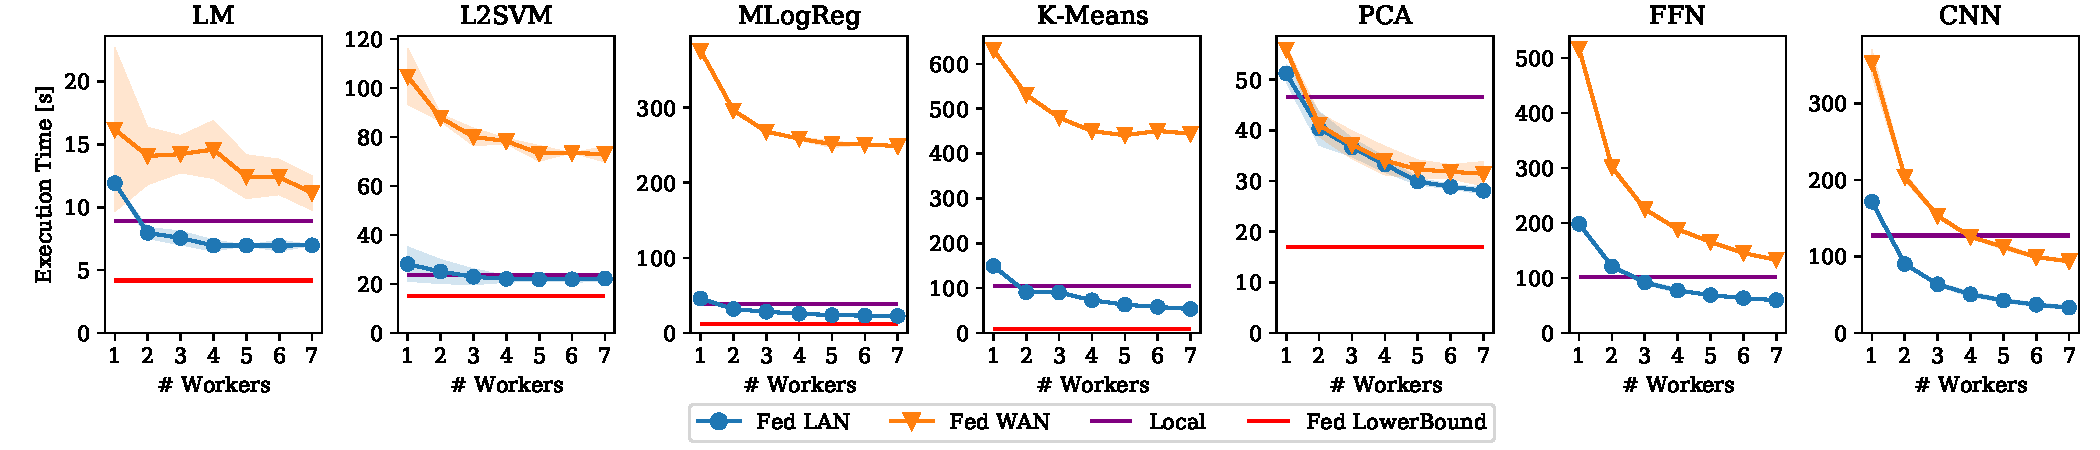
\includegraphics[width=\linewidth]{figures/workers}
	\vspace{-0.25cm}
	\caption{\label{fig:exp1}Basic Algorithm Comparison and Scalability 
	with \# Federated Workers ($10^6 \times \num{1050}$ feature matrix $\mat{X}$).}
	\vspace{-0.2cm}
\end{figure*}

%%%%%%%%%%%%%%%%%%%%%%%%%%%%%%%%%%%%%%%%%%%%%%%%%%%%%%%%%%%%%%%%%%%%%%%%%%%%%%%%%%%%%%%%%%%%%%%%%%%%
\section{Experiments}
\label{sec:experiments}

Our experiments study the performance of the described federated runtime backend of SystemDS (Section~\ref{sec:federated}), with various ML algorithms and pipelines, network configurations, and in comparison with local execution and other ML systems.

\subsection{Experimental Setup}
\label{sec:setup}

\textbf{Baselines:} For evaluating the characteristics of federated linear algebra and parameter servers in controlled yet practically relevant scenarios, we compare the following four main baselines:

\begin{itemize}
\item \emph{Local:} Our main baseline is SystemDS with local, in-memory operations, which uses equivalent runtime plans and runtime operations, but executed locally on a single node.
\item \emph{Federated LAN:} The federated runtime backend dispatches runtime operations on federated matrices to the described federated linear algebra operations and parameter server. For Federated LAN, all coordinator and workers nodes are part of a local area network (LAN) of two racks, connected via an HPE FlexFabric5710 48XGT switch.
\item \emph{Federated WAN:} In addition to Federated LAN, we experiment with the federated backend in a wide-area network (WAN) setting. Here, a client node runs the coordinator in Copenhagen, Denmark and the workers run in a cluster (described below) in Graz, Austria -- a distance of more than $\num{1000}\,\text{km}$ with round-trip latency of about $35$-$60\ms$, and data transfer bandwidth of about $1.4$-$2\mbs$.
\item \emph{Other ML Systems:} To ensure that \emph{Local} is a competitive baseline, we also compare with local execution in Scikit-learn 0.23 \cite{PedregosaVGMTGBPWDVPCBPD11} for traditional batch ML algorithms, and TensorFlow 2.3.1 \cite{AbadiBCCDDDGIIK16} for mini-batch neural network workloads. These systems do not support federated ML. %and thus, do not allow a direct comparison of federated algorithms
\end{itemize}

\textbf{Cluster Configuration:} We ran all experiments described here on eight nodes, each having a single AMD EPYC 7302 CPU at $3.0{-}3.3$\,GHz (16 physical/32 virtual cores), $128\gb$ DDR4 RAM at 2.933\,GHz balanced across 8 memory channels, $2\times 480\gb$ SATA SDDs (system), $12\times 2\tb$ SATA HDDs (data), and $2\times 10\text{Gb}$ Ethernet. The nominal peak performance of each node is $768\gflops$ and $183.2\gbs$, whereas we measured $109.6\gbs$ for an $8\gb$ matrix-vector multiplication. For wide-area network tests, we use an additional client node Dell XPS 15 with one Intel i9-9980HK CPU at $2.4{-}5.0$\,GHz (8 physical/16 virtual cores), and $32\gb$ DDR4 RAM at 2.666\,GHz. Our software stack comprises Ubuntu 20.04.1 as operating system, OpenJDK Java 1.8.0\_265, and SystemDS 2.0.0++ (as of 03/2021), configured with native Intel MKL BLAS for dense matrix-matrix multiplications. The coordinator and worker nodes use consistent JVM configurations of \texttt{-Xmx110g -Xms110g -Xmn11g}, while the WAN client uses \texttt{-Xmx30g -Xms30g -Xmn3g}. 
%REMARK SB: i had to switch to 40g for the parameterServer experiments. + some swap space

\textbf{Workloads:} The tested workloads include the ML algorithms linear regression (LM), $L_2$-regularized support vector machine (L2SVM) and multi-class logistic regression (MLogReg) for classification, K-Means for clustering (with K=50 centroids), principal component analysis (PCA) for dimensionality reduction (with K=10 projected features), as well as two parameter server models: a fully-connected feed-forward network (FFN) with BSP, 5 epochs, batch size 512, and trained with stochastic gradient decent (SGD) with Nesterov momentum, as well as a convolutional neural network (CNN) with BSP, 2 epochs, batch size 128, and standard SGD. These algorithms are trained on a synthetic $1\text{M} \times \num{1050}$ feature matrix (after one-hot encoding categorical features), which closely resembles the characteristics of the data from our paper production use case described in Section~\ref{sec:paper}. For the CNN scenario though, we use the standard $60\text{K}/10\text{K}\times784$ MNIST dataset from computer vision. The feature matrix $\mat{X}$ is stored as a row-partitioned, federated matrix with balanced partition sizes at the federated sites (i.e., worker nodes), while the labels $\mat{y}$ are stored at the coordinator node. We fix the number of maximum iterations for iterative ML algorithms and report the end-to-end runtime---including JVM startup and I/O from binary files---as a mean of (at least) three repetitions.

\subsection{ML Algorithms Performance}
\label{sec:algorithms}

In a first set of experiments, we compare the local ML algorithms performance with both Federated LAN and WAN. We also vary the number of federated workers, evaluate communication settings such as SSL encryption, and compare other ML systems.

\textbf{ML Algorithms:} Figure~\ref{fig:exp1} shows the end-to-end runtime of the ML algorithms. As a first step, consider a scenario of three federated workers (the number of workers is varied on the x-axis), which require additional communication but also provide more computational resources. The ML algorithms have different characteristics in that regard. First, LM internally calls an iterative conjugate-gradient LM method (used for $\text{ncol}(\mat{X})>\num{1024}$), where each iteration performs an $\mat{X}^{\top}(\mat{X}\,\mat{v})$ over the federated data. Compared to local, we observe low overhead and already a runtime improvement with three workers. The Fed LowerBound represents the remaining local execution time that is not subject to federated computation and thus, the best Fed LAN could achieve. Second, L2SVM uses two nested while loops, where each outer iteration computes gradients, and the inner loop performs a line search along the gradient. Since the federated $\mat{X}$ is only accessed via matrix-vector and vector-matrix operations in the outer loop, the differences to the local runtimes are much smaller. Third, MLogReg also uses two nested while loops, but each inner iterations performs an $\mat{X}^{\top}(\mat{w}\odot(\mat{X}\,\mat{v}))$ on the federated $\mat{X}$ and accordingly, we see again a solid improvement with three workers. Fourth, a single run of K-Means has a single while loop, which uses more compute-intensive matrix-matrix multiplications as shown in Example~\ref{ex:kmeans}. Fifth, PCA is a non-iterative algorithm and computes an Eigen decomposition of $\mat{X}^{\top}\mat{X}$ and subsequently, projects the data via another matrix multiplication to K=10 features. With large number of rows, the two matrix multiplications dominate the runtime. Both K-Means and PCA accordingly show also substantial improvements compared to local execution. Finally, FNN and CNN use the mini-batch parameter server architecture with local per-batch updates and global per-epoch synchronization. The larger compute resources of the federated backend yield improvements despite the additional communication. Most importantly, none of these federated ML algorithms ever communicates the raw input data to the coordinator (and thus, preserve privacy of the federated data), they all show only small overhead, and in many cases even runtime improvements. In additional experiments with federated labels $\mat{y}$ and/or smaller number of columns (not shown here), we observe that some algorithms like L2SVM incur substantially larger overhead though, because all vector operations of the inner loop are then converted to federated operations as well, which increases communication without benefiting from the larger computational resources. In the Federated WAN setting, the relative communication overhead is also substantially higher, but even there, the end-to-end overhead is  moderate, which renders federated learning practical for real deployments.

\begin{figure}[!t]
	\centering
	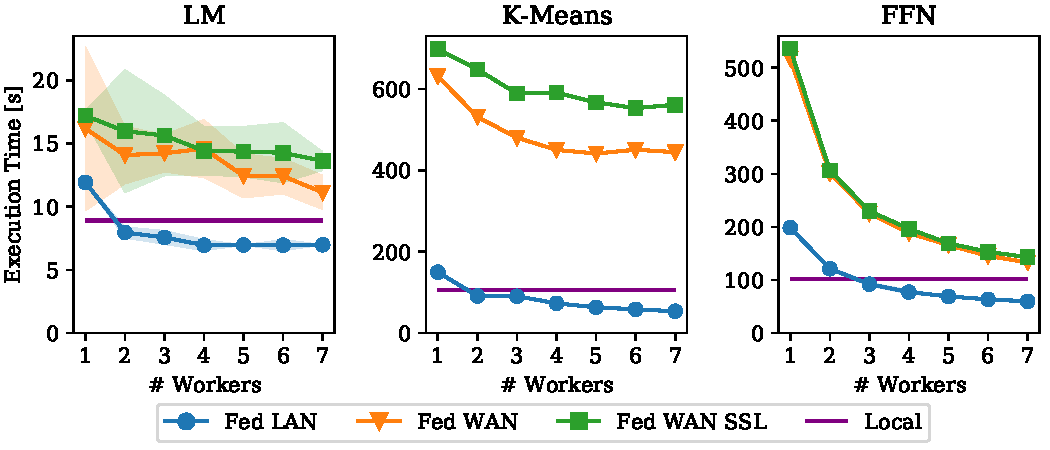
\includegraphics[scale=0.46]{figures/workersSSL}
	\vspace{-0.25cm}
	\caption{\label{fig:exp2}Comparison of Communication Settings.}
	\vspace{-0.1cm}
\end{figure}

\textbf{Scalability:} Besides the comparison of Local, Federated LAN, and Federated WAN, Figure~\ref{fig:exp1} also shows the scalability of our federated backend with increasing number of federated workers. We investigate strong scaling behavior by keeping the data size constant. The coordinator sends federated requests in parallel to all the workers and either broadcasts all side inputs or only relevant slices according to operation requirements. The size of communicated intermediates is moderate in all scenarios though; typically, we exchange only vectors in the number of rows (LM, L2SVM, MLogReg, KMeans) or columns (LM, L2SVM) of $\mat{X}$, columns-by-classes (MLogReg), columns-by-centroids (K-Means), columns-by-columns (PCA), or model sizes (FFN, CNN). Accordingly, we see good scalability, where additional workers even improve the runtime up until a point, where the partitions per worker become so small that communication increasingly dominates the total runtime. For L2SVM and LM, the improvements are smaller because L2SVM is dominated by vector operations at the coordinator, and LM has a very small runtime, where initial startup constitutes a large fraction of total execution time. 
In the Federated WAN, the communication overhead is larger but still moderate overall. As the number of workers increases both federated computation and---maybe surprisingly---communication time reduces. The coordinator sends RPCs to all workers in parallel (which mitigates the additional latency), and the more workers the smaller some of the transferred intermediates (e.g., n/\#workers).

\textbf{SSL Encryption:} As mentioned in Section~\ref{sec:design}, the federated backend of SystemDS supports SSL-encrypted communication channels between the coordinator and federated workers. We leverage Netty's \texttt{SslContext} for encrypting the federated requests and responses including exchanged data. In a next experiment, we study the overhead this encrypted communication entails. Figure~\ref{fig:exp2} compares LM, K-Means, and FFN---which have very different characteristics and thus, showed different scaling behavior---in the Federated LAN, Federated WAN, and Federated WAN with SSL settings. For LM---where exchanged intermediates are small (vectors in the number of columns)---the overhead of WAN and additional SSL encryption is limited to about 2x and 10\%, respectively. K-Means shows larger overhead of about 4-8x in a WAN setting due to more iterations and larger transfers (columns-by-centroids), and again about 15\% overhead for SSL. In contrast, the federated parameter server shows only moderate WAN and SSL overhead because of the higher computational workload per worker and infrequent per-epoch global model updates and synchronization.

\begin{figure}[!t]
	\centering
	\includegraphics[scale=0.47]{figures/mlsystems}
	\vspace{-0.25cm}
	\caption{\label{fig:exp3}Comparison with Other ML Systems.}
\end{figure}

\textbf{ML System Comparison:} With the comparison of local and federated algorithms in mind, we can now turn to a comparison with other ML systems, specifically Scikit-learn \cite{PedregosaVGMTGBPWDVPCBPD11} and TensorFlow \cite{AbadiBCCDDDGIIK16} as widely-used ML systems. We select K-Means, PCA, FFN, and CNN for comparison in order to limit the influence of algorithmic differences. The algorithms were configured to yield a similar number of iterations (e.g., K-Means) and final accuracy. Figure~\ref{fig:exp3} shows the results comparing local and Federated LAN configurations of K-Means and PCA with Scikit-learn, and FFN and CNN with TensorFlow. Overall, we observe mixed results. K-Means is 1.6x slower than Scikit-learn, while PCA is 2x faster. Similarly, FFN is 25\% faster, while CNN is 2x slower than TensorFlow. We attribute these differences to remaining algorithmic discrepancies, and the comparison with best-of-breed ML systems for the different algorithms, whereas SystemDS aims to support a wide range of algorithms and deployments. For CNN, the overhead is partially due to SystemDS using sparse conv2d\_backward data/filter and other operations because MNIST and related intermediates are just below the internal sparsity threshold. Moreover, TensorFlow's parallel operator scheduling is advantageous in small mini-batch scenarios. In additional experiments on a spectrum of data characteristics, we observed relative improvements of SystemDS compared to the other ML systems with increasing sparsity, number of rows, and batch size. Most importantly, these comparisons ground the observed Federated LAN results in a performance range close to state-of-the-art systems, supporting the conclusion of applicability in practice.

\subsection{ML Pipelines Performance}

In a second set of experiments, we now return to our main motivation of supporting entire ML pipelines on federated raw input data without central data consolidation. We evaluate ML pipelines of the use cases described in Section~\ref{sec:usecases} on synthetic data.

\textbf{ML Pipeline Setup:} The workload is a simplified training pipeline P2 of the paper production use case (see Section~\ref{sec:paper}). This pipeline reads the input data of continuous and categorical features as a federated frame, and transforms the frame via recoding and one-hot encoding (see Section~\ref{sec:dataprep}) into a numeric input matrix and a meta frame that holds the recode maps. Subsequently, we perform value clipping for values outside the interval $[-1.5\sigma,1.5\sigma]$ of column standard deviations, normalize the data to zero column means and column standard deviations one, and finally, create 70/30 train and test splits. In order to retain a balanced data distribution across federated workers, we perform this splitting via a uniformly sampled selection-matrix-multiply. Finally, we train a regression or neural network model on the train split, evaluate its performance on the test split, and write out the model and metadata.

\begin{figure}[!t]
	\centering
	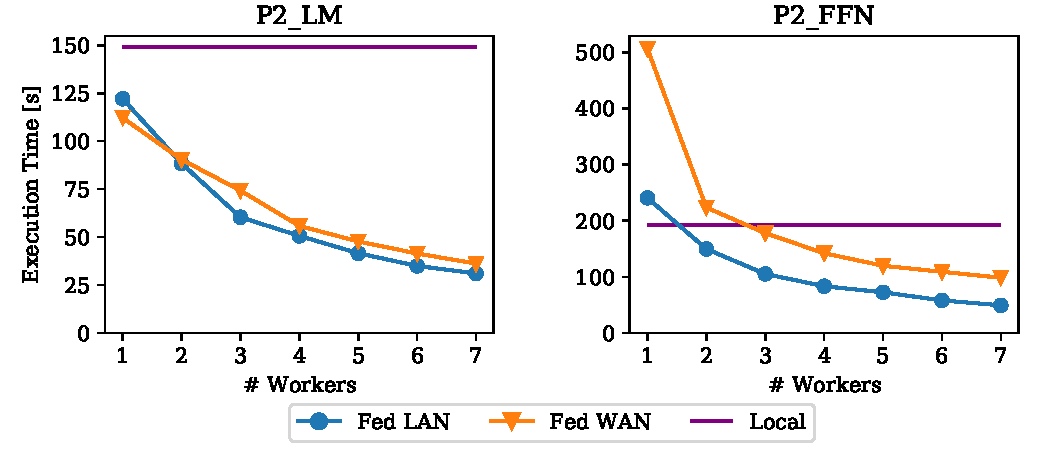
\includegraphics[scale=0.47]{figures/workersPL}
	\vspace{-0.25cm}
	\caption{\label{fig:exp4}ML Pipeline Scalability with \# Federated Workers.}
\end{figure}

\textbf{Scalability:} Figure~\ref{fig:exp4} shows the total execution time of ML pipeline P2 on a synthetic federated dataset of $10^6$ observations that map---after encoding---to a $1\text{M} \times \num{1050}$ feature matrix. As the number of workers increases, we again see good improvements compared to local operations. The federated transformencode, pre-processing like outlier removal and normalization, train/test splitting, and LM training nicely map to federated linear algebra operations. P2\_LM and P2\_FNN differ only in the used training algorithm. The larger compute workload of P2\_FNN then explains the better scalability with more workers. For P2\_LM, already a single worker shows improvements over local execution because of the additional resources of a coordinator and one worker compared to a single node, which can be used for garbage collection and JIT compilation. Finally, we also partially support the remaining ML pipelines of our use cases in a federated environment. These pipelines include pre-processing steps like missing value imputation, PCA, correlation matrices, density-based clustering, as well as the task-parallel training of multiple GMM (Gaussian Mixture Model) instances. 

%%%%%%%%%%%%%%%%%%%%%%%%%%%%%%%%%%%%%%%%%%%%%%%%%%%%%%%%%%%%%%%%%%%%%%%%%%%%%%%%%%%%%%%%%%%%%%%%%%%%
\section{Related Work}
\label{sec:relatedwork}

The ExDRa system is related to existing work of data analysis on raw data, federated learning systems, as well as model and pipeline management. We combine and extend techniques of these areas for exploratory data science workflows on federated raw data.

\textbf{Data Analysis on Raw Data:} Query processing on raw data \cite{AlagiannisBBIA12,IdreosAJA11} processes SQL queries directly on raw input files in order to avoid expensive data loading in the context of exploratory analysis. To alleviate repeated parsing and data access overhead, for example, positional maps and attribute caches are transparently build and exploited during repeated analysis of the same files \cite{AlagiannisBBIA12}. Furthermore, code generation techniques are used to specialize the query engine for heterogeneous input formats \cite{KarpathiotakisA16}. Orthogonal to existing work, we aim to support data pre-processing pipelines and linear algebra programs on such raw data sources. This research direction is also related to different categories of ML systems. First, there are ML systems with good support for multi-modal input features such as DeepDive \cite{ShinWWSZR15}, Overton \cite{Re20}, and Ludwig \cite{abs-1909-07930}; systems for more complex feature extraction, and pre-processing like TFX \cite{BaylorBCFFHHIJK17} and SageMaker \cite{DasIBRGKDRPSWZS20}; and systems for data cleaning like HoloClean \cite{RekatsinasCIR17,HeidariMIR19}, AlphaClean \cite{abs-1904-11827}, BoostClean \cite{abs-1711-01299}, and CPClean \cite{cpclean}. Second, there are ML systems that exploit materialized intermediates for reuse and debugging such as Columbus \cite{ZhangKR14}, Helix \cite{XinMLMSP18}, Collaborative Optimizer \cite{DerakhshanMARM20}, and Mistique \cite{VartakTMZ18}. In contrast to these two categories, we provide system infrastructure for executing and optimizing ML pipelines on federated raw data.
 
\textbf{Federated Learning:} Privacy-preserving ML is a very active research area with major challenges and opportunities. A major direction is the use and specialization of privacy-enhancing technologies such as differential privacy \cite{JiLE14}, fully homomorphic encryption (FHE) \cite{Gentry09,AcarAUC18,GiladBachrachD16}, and secure multi-party computation (MPC) \cite{MohasselZ17}, where FHE and MPC are often only used for inference, that is, scoring private user input \cite{GiladBachrachD16,JuvekarVC18,DathathriS0LLMM19}. In contrast, federated learning broadly aims to learn ML models without central data consolidation and exposing raw input data. Early work on federated or decentralized learning \cite{McMahanMRA16,McMahanMRHA17,LianZZHZL17,BonawitzEGHIIKK19} adopted an architecture similar to traditional parameter servers \cite{SmolaN10,DeanCMCDLMRSTYN12,LiAPSAJLSS14,JiangCZY17}, but augmented this architecture by additional techniques such as client sampling \cite{McMahanMRHA17}, agent-based, fault tolerant, decentralized aggregation \cite{BonawitzEGHIIKK19, BonawitzIKMMPRS17}, peer-to-peer gradient and model exchange \cite{WatcharapichatM16,LianZZHZL17,LianZZL18}, and meta learning for federated, private recommendation models \cite{LinRCRY0RC20,abs-2101-06927}. A major challenge for federated parameter servers is statistical (and hardware) heterogeneity \cite{LiSTS20,Smith20} that can negatively affect convergence \cite{abs-1812-01097}. Recent techniques include reducing variance \cite{TangLYZL18}, selecting relevant subsets of data \cite{tuor2020overcoming}, tolerating partial client work \cite{LiSZSTS20}, partitioning the client population into independent, congruent groups \cite{abs-1910-01991}, and adaptive optimization at the server with standard SGD at the clients \cite{abs-2003-00295}. For such algorithmic improvements, also new benchmarks such as LEAF \cite{abs-1812-01097} are emerging.

\textbf{Federated Learning Systems:} In contrast to algorithmic work on federated learning, infrastructure for federated learning is relatively sparse, and includes agent-based federated (parameter) servers \cite{BonawitzEGHIIKK19}, and systems that rely on privacy-enhancing technologies tailored for specific algorithms such as tree-based models \cite{WuCXCO20}. A careful reader might wonder if work on in-DBMS ML \cite{LuoGGPJ17,JankovLYCZJG19,DsilvaMK18} could be combined with traditional federated query processing \cite{JosifovskiSHL02} through wrappers, external tables, or SparkSQL's data sources \cite{ArmbrustXLHLBMK15}. While conceptually possible, the wrappers would need to allow the push down of partial linear algebra operations, and the federated sources would also require a linear algebra and parameter server runtime. More relevant to federated learning, TensorFlow Federated (TFF) \cite{tff,Smith20} recently provides high-level primitives such as \texttt{tff.federated\_broadcast}, \texttt{tff.federated\_map}, and \texttt{tff.federated\_mean} for composing federated computation. This TFF API shares design aspects with our federated backend (at a higher level than our federated requests), but is at a much lower level than linear algebra programs, focuses primarily on simulating federated environments, and an open-source federated device runtime does not exist yet. In contrast to such dedicated APIs, we aim to support federated data preparation, parameter servers, and linear algebra programs via automatic plan generation, and thus, a wide variety of existing algorithms and higher-level primitives without the need for users to implement federated learning. 

\textbf{Model and Pipeline Management:} The model and pipeline management components in ExDRa are related to several subareas. First, ML pipeline management in Columbus~\cite{ZhangKR14}, KeystoneML~\cite{SparksVKFR17}, and TuPaQ~\cite{SparksTHFJK15} similarly aim to remove unnecessary redundancy in feature selection and hyper-parameter tuning workloads. Second, recent frameworks like MLflow~\cite{ChenCDD0HKMMNOP20,ZahariaCD0HKMNO18} and ModelDB~\cite{VartakM18} also provide catalogs and repositories of pipelines and models, experiment tracking, and related provenance information. Third, AutoML tools like Auto-WEKA~\cite{ThorntonHHL13}, Auto-WEKA 2.0~\cite{KotthoffTHHL17}, Auto-sklearn~\cite{FeurerKES0H19}, TPOT~\cite{OlsonM19}, Alpine Meadow~\cite{ShangZBKECBUK19}, Amazon SageMaker Autopilot~\cite{DasIBRGKDRPSWZS20}, and other AutoML cloud services (e.g., Azure ML, Google AutoML) \cite{ZhangZWZ17} provide means of pipeline recommendations. Beyond state-of-the-art, ExDRa focuses on data science workflows on federated raw data, and pipeline recommendations that offer good accuracy-runtime tradeoffs in this challenging context.

%%%%%%%%%%%%%%%%%%%%%%%%%%%%%%%%%%%%%%%%%%%%%%%%%%%%%%%%%%%%%%%%%%%%%%%%%%%%%%%%%%%%%%%%%%%%%%%%%%%%
\section{Conclusions}

To summarize, we gave an overview of the ExDRa system for exploratory data science on federated raw data. We described use cases, deployment and privacy models, the system architecture, selected features of SystemDS' federated runtime backend, and promising experimental results. Compared to local ML training, federated linear algebra programs and federated parameter servers exhibit only small to moderate overhead (and can even improve the runtime). At the same time, federated learning preserves the privacy of federated raw data via practical means such as aggregates and encrypted communication. In conclusion, federated learning shows great promise for broad applicability in practice. The automatic generation of federated execution plans then allows reusing and deploying a wide variety of ML algorithms, as well as data preparation and model debugging techniques in such federated environments. However, a deployment in a multi-company context further requires a trusted system infrastructure, and means of generating and verifying federated execution plans under awareness of privacy constraints. Beyond this hardening of the infrastructure, we see many opportunities for future work, especially regarding ML pipelines on federated raw data, a fine-grained spectrum of privacy enhancing technologies with different tradeoffs, and self-balancing incentives for participating federated sites.


%%%%%%%%%%%%%%%%%%%%%%%%%%%%%%%%%%%%%%%%%%%%%%%%%%%%%%%%%%%%%%%%%%%%%%%%%%%%%%%%%%%%%%%%%%%%%%%%%%%%
\section*{Acknowledgements}
The ExDRa project is funded through the bilateral program ``ICT of the Future -- Smart Data Economy" by the German Federal Ministry for Economic Affairs and Energy (BMWi, 01MD19002), and the Austrian Federal Ministry for Climate Action, Environment, Energy, Mobility, Innovation and Technology (BMK, 873838). Additional contributions by Sebastian Benjamin Wrede were made within the Know-Center GmbH, DDAI COMET module (funded by BMK, BMDW, FFG, SFG, and industrial partners). Furthermore, we also thank Arnab Phani, David Weissteiner, and Valentin Leutgeb for their valuable contributions to the implementation of SystemDS' federated backend, as well as our anonymous reviewers for their constructive criticism, comments, and suggestions.

%%%%%%%%%%%%%%%%%%%%%%%%%%%%%%%%%%%%%%%%%%%%%%%%%%%%%%%%%%%%%%%%%%%%%%%%%%%%%%%%%%%%%%%%%%%%%%%%%%%%
\balance
\bibliographystyle{ACM-Reference-Format}
\bibliography{SIGMOD2021}
  
\end{document}
\endinput
